\documentclass[conference]{IEEEtran}

% =========================================================
% PACKAGES
% =========================================================
\usepackage[T1]{fontenc}
\usepackage{cite}
\usepackage{amsmath,amssymb,amsfonts}
\usepackage{graphicx}
\usepackage{xcolor}
\usepackage{booktabs}
\usepackage{multirow}
\usepackage{array}
\usepackage{tabularx}
\providecommand{\makecell}[2][c]{\begin{tabular}[#1]{@{}#1@{}}#2\end{tabular}}
\usepackage{url}
\usepackage{balance}
\usepackage{enumitem}

% =========================================================
% PAPER METADATA
% =========================================================
\title{Task-Adaptive Architecture Optimization for LLM-Based Multi-Agent Systems via Reinforcement Learning and Dynamic Graph Construction}


\author{
\IEEEauthorblockN{Naveen Tanikonda}
\IEEEauthorblockA{\textit{Computer Science and Engineering} \\
\textit{VIT-AP University}\\
Amaravati, India \\
naveen.23bce9787@vitapstudent.ac.in}
\and
\IEEEauthorblockN{VeeraBhadra Jagarlamudi}
\IEEEauthorblockA{\textit{Computer Science and Engineering} \\
\textit{VIT-AP University}\\
Amaravati, India \\
bhadra.23bce9780@vitapstudent.ac.in}
\and
\IEEEauthorblockN{Sriram Somarouthu}
\IEEEauthorblockA{\textit{Computer Science and Engineering} \\
\textit{VIT-AP University}\\
Amaravati, India \\
sriram.23bce20270@vitapstudent.ac.in}
\and
\IEEEauthorblockN{Ravi Teja Perumalapalli}
\IEEEauthorblockA{\textit{Computer Science and Engineering} \\
\textit{VIT-AP University}\\
Amaravati, India \\
teja.23bce9392@vitapstudent.ac.in}
\and
\IEEEauthorblockN{Dr. Srinivasa Rao Pokuri\textsuperscript{*}}
\IEEEauthorblockA{\textit{Senior Assistant Professor} \\
\textit{School of Computer Science and Engineering} \\
\textit{VIT-AP University}\\
Amaravati, India \\
Contact: +91 9491860686 \\
Email: pokuri.srinivasarao@vitap.ac.in}
}

\thanks{\textsuperscript{*}Corresponding author.}

\IEEEoverridecommandlockouts

\begin{document}
\maketitle

% =========================================================
% ABSTRACT
% =========================================================
\begin{abstract}
Large Language Model Multi-Agent Systems permit several specialised agents to cooperate with each other to accomplish difficult tasks, like reasoning, coding and information retrieval. Traditional multi-agent systems often employ static topologies, where all the tasks consist of the same set of agents. As a result, the overheads, costs, delays in the processing in sequence and inference cost for a simple query increase. This paper proposes the task-conditional solution for topology optimisation for multi-agent systems which is based on Large Language Models (LLMs). It enables the system to choose which agents to employ, the function of each one of them, and the communication pattern of agents among each other. Multi-agent topology selection can be viewed as a Markov Decision Process (MDP) task. Two significant contributions are proposed in this paper. First of them is the real-time active tabular Q-Learning selector, invariant architecture manager and dynamic state graph compiler (C2).Using a benchmark of 18 tasks in 6 different domains, the Q-Learning selector has been able to reduce the total tokens required by 60.46\%(p=0.0031). The amount required for inference has been reduced from \$0.31662 to \$0.12517, which is consistent with the token reduction that was achieved theoretically (36.19\%). The Q-Learning selector is also able to reduce the number of agents required (pruning) by 50.0\% from a selection of 6 master agents, (or 40.0\% of the 5) selection of master agents. The critical path length has been reduced from 5.00 to 2.89(-42.2\%, t=19.00, p=6.91x10-13). The Q-Learning selector still retains the ability to complete 100\% of the tasks (16 out of 18) with a macro mean of 94.44\%. The Q-Learning selector has a dynamic compilation delay of below 15ms. Second, we explore the ability to incorporate neural adaptation into a common policy learnt across various different tasks in multi-agent task-conditional scenarios (C1). We have found that in discrete action space (planning and analysis), the neural adaptation provides no additional benefits in terms of improvement on 4 tasks. Neural adaptation provides a protective mechanism while doing summarization tasks.
\end{abstract}

\begin{IEEEkeywords}
Multi-agent systems, large language models, reinforcement learning, adaptive architecture, dynamic workflows, state-graph compilation, graph pruning, critical path compression.
\end{IEEEkeywords}

% =========================================================
% 1. INTRODUCTION
% =========================================================
\section{Introduction}
\label{sec:introduction}

Large Language Models (LLMs) have exhibited their prowess in a number of tasks ranging from NLU, mathematical reasoning, code generation, and more. Benchmarking systems like the AgentBench~\cite{liu2024agentbench} showcase how LLMs can be benchmarked through their performance as autonomous agents in different environments. Single-agent prompting is not scalable and thus collaborative Multi-Agent Systems (MAS) are state-of-the-art for solving complex decomposition tasks. There are a few standardized steps to collaboration in MASs~\cite{hong2024metagpt, wu2023autogen, qian2024chatdev}. Each of these agents plays certain specific roles, and some examples include planning, research, code generation, critique, and result generation among others.

Traditional multi-agent systems for LLMs have the issue of \emph{ rigid structure }.
Current multi-agent systems follow a static execution structure.
The complete multi-agent system is used to solve any problem irrespective of the complexity of the problem.
It doesn’t matter whether it’s a simple task such as a greeting or a calculation or a complex one such as a distributed system design.
All of them will make use of the same multi-agent system.
This leads to unnecessary extra processing due to the entire planning, research, coding and verification process.
\begin{enumerate}[leftmargin=*]
    \item \textbf{Token Usage & Cost:} Unnecessary specialised agents result in superfluous context windows, hence more token usage and API costs.
    \item \textbf{Latency & Bottlenecking:} Linear and dense pipelines require sequential execution of the agents involved. This implies that the latency will depend on the number of agents in the pipeline rather than the complexity of the task ~\cite{Li2025AdaptiveGraphPruning}.
    \item \textbf{Noise & Hallucination:} Extra agent calls at intermediate stages lead to noise in your context, hence hallucinations ~\cite{xiao2026agentdropout}.
\end{enumerate}

\begin{figure*}[!t]
\centering
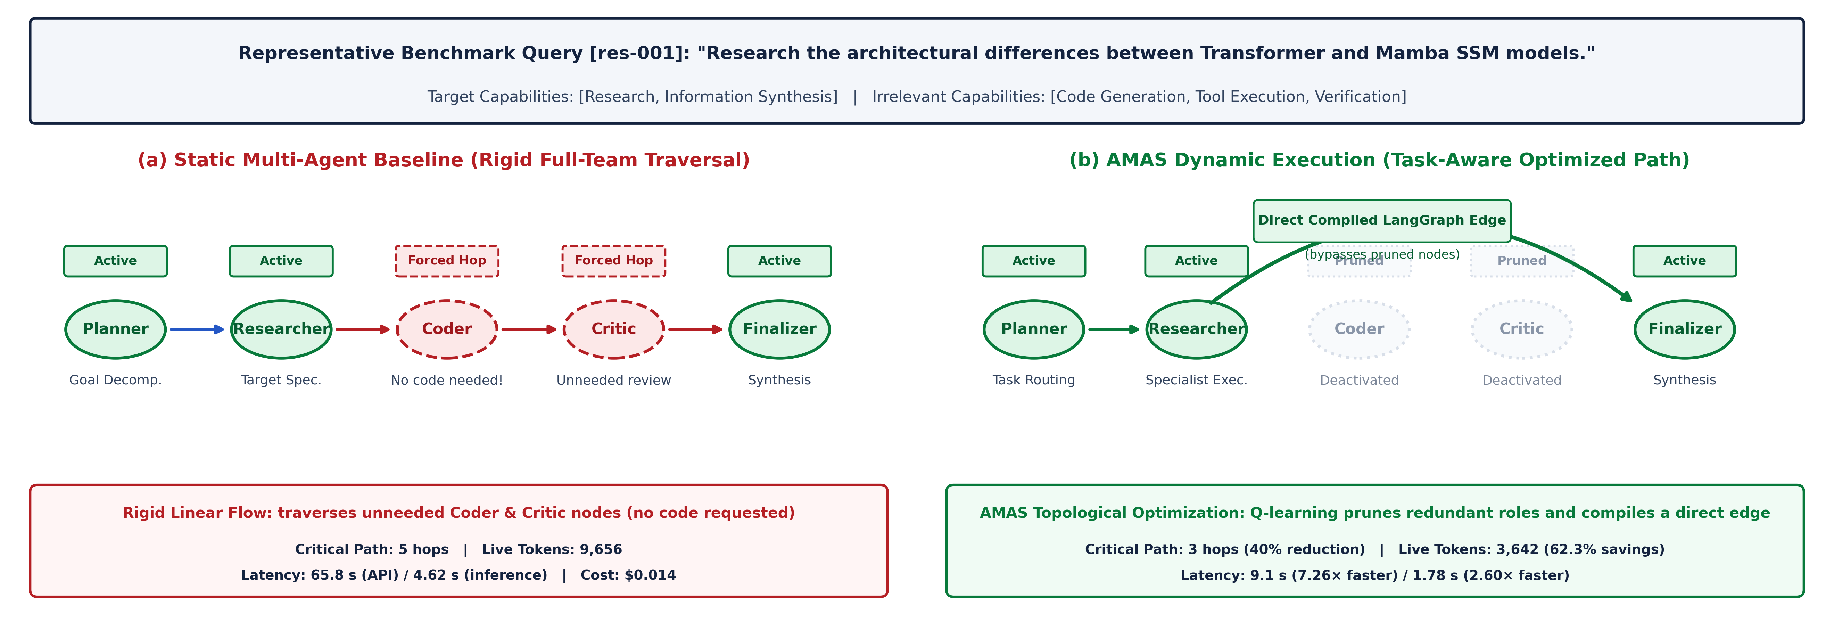
\includegraphics[width=0.96\textwidth]{figures/figure_02_dynamic_topologies.pdf}
\caption{Task-adaptive multi-agent execution example using Res-01 benchmark query (``Investigate architectural distinctions between Transformer and Mamba SSM models''). (a) Static multi-agent approach runs full 5-agent pipeline linearly, including superfluous Coder and Critic ($L_{\mathrm{crit}} = 5$ hops, 9,656 tokens, 65.8\,s end-to-end endpoint latency; 4.62\,s estimated unqueued inference). (b) AMAS adapts on-the-fly by recognizing necessary skills, pruning unnecessary agents, and creating shortcut edge directly from Researcher to Finalizer ($L_{\mathrm{crit}} = 3$ hops, 3,642 tokens, 62.3\% token savings, 9.1\,s endpoint latency [7.26$\times$ speedup]; 1.78\,s unqueued inference [2.60$\times$ speedup]).}
\label{fig:dynamic_topologies}
\end{figure*}

Several approaches have been introduced recently to tackle the above problems, such as dynamic topological optimization, communication graph pruning, and adaptive agent selection~\cite{liu2024dylan,zhuge2024gptswarm,zhang2024aflow,Zhang2025MaAS,Li2025AdaptiveGraphPruning,xiao2026agentdropout,zhang2025gdesigner}. As depicted in Fig.~\ref{fig:dynamic_topologies}, using static multi-agent pipelines leads to the use of some unnecessary intermediate agents to execute queries (e.g., Coder and Critic in order to generate an answer for a research question) which results in token wastage. The proposed AMAS pipeline is able to dynamically identify the required skills and prune unnecessary nodes and edges in order to reduce the critical path to 3 hops from 5 hops.In addition, the model significantly decreases the total token consumption of the entire benchmark suite of 18 problems by 60.46\% and reduces the runtime of processed queries by 7.26$\times$ at real API endpoints ($9.1$\,s vs $65.8$\,). The un-queued inference time is also reduced by 2.60$\times$ because of the decrease in the number of hops ($1.78$\,s vs $4.62$\,). Methods in the literature have high computational overheads, DyLAN~\cite{liu2024dylan} needs multi-round peer score computation, AFlow~\cite{zhang2024aflow} has 15-30 Monte Carlo Tree Searches. MaAS~\cite{Zhang2025MaAS} also has heavy pre-processing overhead of generating the supernet by evolution.

Inspired by recent developments in LLMs, the paper deals with the issue of designing adaptable architectures for LLM-based multi-agent systems via reinforcement learning. This paper makes contributions to the following aspects:

\textbf{Contribution 1 (C1: Experimental Neural Pathway):} We assess the effectiveness of task-conditioned policy that is adapted based on the neural network that was learned on a distribution of task environments. The policy uses the concatenation of task and state embeddings as input and produces modification scores of the architecture. The policy is compared with the scratch initialization and deterministic algorithm and random policies in a comprehensive multi-seed experiment. We keep the negative results with respect to our network architecture, looking into why the action space is too small for capability recovery. The policy is executed in a deterministic compatibility proxy and not during runtime.

\textbf{Contribution 2 (C2: Live Runtime Q-Learning Pipeline):} The Q-Learning Pipeline is a fully-fledged, end-to-end, adaptive runtime system that employs task-aware tabular Q-learning for optimizing multi-agent execution topologies for each individual query. The system makes different changes to the graph topology. A graph invariant manager guarantees that the modifications made will be valid (turning agents on/off, making new edges/edge removals, etc.). Finally, logical topologies are compiled into a valid stateful computation graph in less than 15\,ms, enabling conditional routing and quality reroutes.

Three research questions can be formulated:
\begin{itemize}[leftmargin=*]
    \item \textbf{RQ1 (Topological Efficiency):} Can a RL agent do sparsity pruning in order to minimize the number of redundant agents and execution path size, while having full capability coverage?
    \item \textbf{RQ2 (Runtime Compilation Overhead):} Is it possible to generate and compile a dynamic multi-agent graph without causing overhead to the LLM inference?
    \item \textbf{RQ3 (Cross-Task Knowledge Transfer):} Will the neural policy benefit from pre-training the policy across multiple tasks?
\end{itemize}

The remainder of this paper is organized as follows. First, related works are discussed in Section \ref{sec:related_work}. The problem statement and evaluation metrics are discussed in Section \ref{sec:problem_formulation}. Section \ref{sec:architecture} covers the design of the system. Section \ref{sec:neural_adaptation} covers the neural adaptation (C1). Section \ref{sec:runtime_q_learning} covers the Q-learning and graph compilation (C2). Section \ref{sec:experimental_setup} covers the benchmark and experimental setup. Section \ref{sec:experimental_results} covers the experimental results. Section \ref{sec:statistical_analysis} covers the inferential statistics results. Section \ref{sec:discussion} and Section \ref{sec:limitations} cover the discussion and limitations. Finally, the conclusion can be found in Section \ref{sec:conclusion}.

% =========================================================
% 2. RELATED WORK
% =========================================================
\section{Related Work}

\label{sec:related_work}

\subsection{Static vs. Dynamic Multi-Agent Architectures}

Multi-agent collaboration allows a group of special language models to collaborate to solve complex problems. MetaGPT~\cite{hong2024metagpt}, AutoGen~\cite{wu2023autogen}, and ChatDev~\cite{qian2024chatdev} show how stable reasoning becomes due to having SOPs and roles. Nevertheless, they are \textit{static systems}, which means all requests will be solved using the same pipeline. Budget-aware approaches, such as BAMAS~\cite{Yang2026BAMAS}, orchestration~\cite{dang2025multiagent}, and AgentNet~\cite{yang2025agentnet} have demonstrated how flexible topology and evolving agents can help to decrease the cost. AgentDropout~\cite{xiao2026agentdropout} demonstrates how unnecessary agents can be turned off. DyLAN~\cite{liu2024dylan} uses an unsupervised rating approach to exclude unneeded agents. However, there is an $\mathcal{O}(N^2)$ cost of rating prompts, which makes this solution inefficient for simple requests.

\subsection{Graph Architecture Search, Optimization, and Pruning}

Flexibly topology is another interesting topic when it comes to multi-agent systems. GPTSwarm~\cite{zhuge2024gptswarm} showed how one can express ensemble using differentiable graph. It uses reinforcement learning to optimize the weights of the connections between agents. But it still keeps the fully connected topology. AFlow~\cite{zhang2024aflow} showed how to automatically generate workflow using MCTS (Monte Carlo Tree Search). This is because the agents were responsible for generating code. This proved that the workflow can be made task specific. Multi-agent architecture search~\cite{Zhang2025MaAS} showed the use of agents in order to search for an optimal role and edges inside of super-architecture using evolutionary approach. The work of CARD/AGP~\cite{Li2025AdaptiveGraphPruning} reduces critical path by 44\% (5.0 to 2.8 hops).

Recently, there has been work on how to design flexible topologies. G-Designer~\cite{zhang2025gdesigner} uses variational graph auto encoders to design flexible communication topologies depending on tasks. AgentConductor~\cite{wang2026agentconductor} examines how to evolve topologies for code generation at competition level. NeuralFSM~\cite{wang2026neuralfsm}, shows how to use neural FSMs for flexible coordination. Jiang et al.~\cite{Jiang2026GTD} study how graphs can be used for diffusion models for designing communication topologies. Agent Q-Mix~\cite{jiang2026agentqmix} uses multi-agent value decomposition for action selection. MetaAgent-X~\cite{Zhang2026MetaAgentX} uses end-to-end reinforcement learning for automated multi-agent systems design. AMAS leverages this by employing sub-millisecond Q-learning with guaranteed topologies. DAGs are converted to state graphs (using LangGraph~\cite{langgraph2024}) and can be constructed with less than 15\,ms overhead.

\subsection{Reinforcement Learning for LLM Multi-Agent Collaboration}

Recently, reinforcement learning has been gaining relevance as one of the methods that could be applied to multi-agent coordination through large language models. Liu et al.~\cite{liu2026llm} have created collaborative multi-agent reinforcement learning for LLMs. Zhao et al.~\cite{Zhao2026StrongerMAS} presented Stronger-MAS and demonstrated how multi-agent reinforcement learning could be applied for collaborative alignment. The OptAgent~\cite{bi2025optagent} framework uses verbal reinforcement learning to enhance communication between agents and debate consistency. ReMA~\cite{Wan2025ReMA} use MARL for meta-thinking in order to decrease multi-agent deliberation. Meta-policies for multi-agent collaboration are studied by Yang and Thomason~\cite{Yang2026LearningToDeliberate}. ResMAS~\cite{Zhou2026ResMAS} introduce resilient optimization. Rjoub~\cite{rjoub2026aamc} introduces adaptable meta controllers.

\subsection{Meta-Reinforcement Learning and Cross-Task Transfer}

Meta-RL focuses on the learning of generalizable strategies for adaptation in various tasks~\cite{Huang2024AdaptiveMARL,Kashikar2025MetaRL}. Contextual meta MARL involves cooperation of different agents with varying properties in their teams~\cite{Huang2024AdaptiveMARL}. Kashikar~\cite{Kashikar2025MetaRL} study emergent communication for zero-shot coordination. Fu et al.~\cite{Fu2026MOFA} study orthogonal expert mixtures (MOFA) for fast transfer. Zhang et al.~\cite{zhang2025bilevel} propose bi-level knowledge transfer for multi-task MARL. The self-play approach to meta-RL has been studied for decentralized multi-agent systems~\cite{Mali2026SelfPlay,li2020adaptive}. Literature surveys~\cite{Cao2025TNNLSSurvey,sun2024llmmarl,lee2026survey} show the pressing need to cut down token waste in multi-agent systems. We have studied in our experiments (C1) how neural policies trained on different tasks via synthetic tasks can generalize.

Table~\ref{tab:literature_comparison}represents a comparison between our system and some of the literature. The rows represent the criteria, while the columns represent the systems. AMAS capabilities and the empirical limitations are indicated in bold.

\begin{table*}[!t]
\centering
\caption{Systematic Comparison with Related Dynamic Multi-Agent Architectures (Features in Rows, Frameworks in Columns)}
\label{tab:literature_comparison}
\footnotesize
\setlength{\tabcolsep}{3.0pt}
\renewcommand{\arraystretch}{1.22}
\begin{tabularx}{\textwidth}{>{\raggedright\arraybackslash\bfseries}p{2.85cm} *{5}{>{\raggedright\arraybackslash\hyphenpenalty=10000\hsize=0.86\hsize}X} >{\raggedright\arraybackslash\hyphenpenalty=10000\hsize=1.70\hsize\bfseries}X}
\toprule
\makecell[c]{\textbf{Feature /}\\\textbf{Dimension}} & 
\makecell[c]{\textbf{DyLAN}\\\cite{liu2024dylan}} & 
\makecell[c]{\textbf{GPTSwarm}\\\cite{zhuge2024gptswarm}} & 
\makecell[c]{\textbf{AFlow}\\\cite{zhang2024aflow}} & 
\makecell[c]{\textbf{MaAS}\\\cite{Zhang2025MaAS}} & 
\makecell[c]{\textbf{CARD}\\\cite{Li2025AdaptiveGraphPruning}} & 
\makecell[c]{\textbf{AMAS}\\\textbf{(Ours)}} \\
\midrule
Adaptation Method & 
\textbf{Unsupervised peer rating} & 
\textbf{Graph policy grad.} & 
MCTS code rollout & 
Genetic search & 
Contextual bandit & 
\makecell[l]{\textbf{Tabular Q-Learning (Runtime);}\\\textbf{Neural Policy (Offline Exp.)}} \\

Decision Latency & 
$\mathcal{O}(N^2)$ LLM calls & 
Iterative LLM prompts & 
15--30 rollouts & 
Offline evolution & 
\textbf{$<10$\,ms routing} & 
$<1$\,ms lookup (0 tokens) \\

Workflow Compilation & 
Layered agent stack & 
\textbf{Continuous edge weights} & 
\textbf{Python code synthesis} & 
Static specialist DAG & 
Routing DAG & 
Executable State-Graph DAG \\

Active Agent Pruning & 
25--40\% & 
None (fixed team) & 
None (fixed team) & 
18--32\% & 
None (full team) & 
50.0\% (Pool) / 40.0\% (Base) \\

Critical Path Reduction & 
None & 
None & 
Variable & 
None & 
\textbf{44.0\% ($5.0 \to 2.8$ hops)} & 
42.2\% ($5.0 \to 2.89$ hops) \\

Empirical Token Savings & 
15--25\% & 
Negative (utility focus) & 
Negative (MCTS cost) & 
18--32\% & 
Not reported & 
+60.46\% (Production LLM) \\

Cross-Task Transfer & 
No & 
Task-specific & 
No & 
No & 
Tabular only & 
Evaluated on 5 held-out tasks \\
\midrule
Primary Limitation & 
Deliberation token blowup & 
High training sample cost & 
Search latency per query & 
Static offline deployment & 
Heuristic bandit only & 
Restricted action space ($\Delta Q = 0$ on 3 tasks); composite task under-engineering \\
\bottomrule
\end{tabularx}
\end{table*}


% =========================================================
% 3. PROBLEM FORMULATION
% =========================================================
\section{Problem Formulation}
\label{sec:problem_formulation}

\subsection{Model of Multi-Agent System}
Let us assume that the multi-agent system is modeled by means of a directed graph
\begin{equation}
G = (V, E).
\end{equation}
Here $V = \{v_1, v_2, ..., v_n\}$ is a set of specialized vertices (nodes) or agents and $n=|V|$. $E \subset V \times V$ is a set of communication or execution edges. For the considered research, we have 6 possible agents:
\begin{equation}
V = \{\text{Planner}, \text{Tool}, \text{Researcher}, \text{Coder}, \text{Critic}, \text{Finalizer}\}.
\end{equation}

For each step $t$, the active architecture is given by:
\begin{equation}
G_t = \langle \mathbf{v}t, \mathbf{r}t, \mathbf{A}t \rangle
\end{equation}
Where:
\begin{itemize}[leftmargin=*]
\item $\mathbf{v}_t \in \{0, 1\}^n$ is the vector of active agents (agent $i$ is active if $v_{t,i} = 1$).
\item $\mathbf{r}_t = [r_{t,1}, ..., r_{t,n}]$ is the vector of discrete roles assigned to each agent $i$. These roles are taken from a list of available roles $\mathcal{R}$.
\item $\mathbf{A}_t \in \{0, 1\}^{n \times n}$ is a matrix indicating the directed edges between nodes (if $A_{t,ij} = 1$ then agent $i$ can communicate with agent $j$).
\end{itemize}

\subsubsection{Context of Task and the Goal of Optimization}

The user task query can be described as:

\begin{equation}
\mathbf{c}_t = \langle \kappa_t, d_t, \mathcal{C}_t, \mathbf{f}_t \rangle
\label{eq:context}
\end{equation}

where $\kappa_t$ represents the task type, $d_t \in \{1,..., 5\}$ the difficulty of the task, $\mathcal{C}_t \subseteq \mathcal{C}_{all}$ the set of capabilities that allows for performing the task, and $\mathbf{f}_t$ the task context attributes.

The problem is then to design the optimal architecture $G_t^*$ to perform the task $c_t$, optimizing for the net utility under the Pareto framework:
\begin{equation}
G_t^* = \arg\max_{G \in \mathcal{G}_{\mathrm{valid}}}
U_{\mathrm{pareto}}(G, \mathbf{c}_t)
\label{eq:optimization}
\end{equation}
Where $\mathcal{V}(G) = True$ defines valid architectures.

\subsection{Multi-Objective Evaluation Metrics}
The following metrics are used to evaluate how good the architecture is.

\textbf{1) Capability Coverage (C cov)}
It determines whether the active agents along with their associated capabilities cover all the necessary capabilities to do the job.
\begin{equation}
C_{\mathrm{cov}}(G_t, c_t) = \frac{|\mathcal{C}_t \cap \mathcal{C}_{\mathrm{active}}(G_t)|}{|\mathcal{C}_t|} \times 100\%
\end{equation}
Where $\mathcal{C}_{active}(G_t)$ refers to the combination of capabilities possessed by the active agents $\mathbf{v}_t$.

\textbf{2) Agent Pruning Rate (APR)}
This measures the simplicity of the architecture. Here we formally introduce three different types of APRs since there has been a lot of confusion about what APR was in the past research literature:
\begin{align}
\mathrm{APR}_{\mathrm{pool6}}(\mathbf{v}t) & = \frac{6 - \|\mathbf{v}_t\|_1}{6} \times 100\%, \label{eq:apr_pool6} \\ 
\mathrm{APR}_{\mathrm{base5}}(\mathbf{v}t) & = \frac{5 - \|\mathbf{v}_t\|_1}{5} \times 100\%, \label{eq:apr_base5} \\
\mathrm{APR}_{\mathrm{invoked}}(G_t) & = \frac{6 - |V_{\mathrm{invoked}}|}{6} \times 100\%. \label{eq:apr_invoked}
\end{align}
Equation~\eqref{eq:apr_pool6} evaluates pruning with respect to the master list of agents (6 agents), while Equation~\eqref{eq:apr_base5} evaluates it with respect to the static list (5 agents). Finally, Equation~\eqref{eq:apr_invoked} is the number of invoked agents.

\textbf{3) Critical Path Length (L crit)}
Critical path length from start node (Planner) to end node (Finaliser):
\begin{equation}
L_{\mathrm{crit}}(G_t)
=
\max_{p \in \mathcal{P}(\mathrm{Planner} \rightarrow \mathrm{Finalizer})}
|p|_{\mathrm{nodes}}
\label{eq:critical_path}
\end{equation}
The minimal number of steps hence latencies~\cite{Li2025AdaptiveGraphPruning}.

\textbf{4) Pareto Net Utility (U pareto)}
This metric reflects the balance between capability coverage and the tokens consumed.
\begin{equation}
U_{\mathrm{pareto}}
=
0.5 \left(1 - \frac{T_{\mathrm{adapt}}}{T_{\mathrm{base}}}\right)
+
0.5 \left(\frac{C_{\mathrm{cov}}}{100}\right)
\label{eq:pareto_utility}
\end{equation}
where $\mathcal{P}(\mathrm{Planner} \rightarrow \mathrm{Finalizer})$
denotes the set of all directed paths from the Planner to the
Finalizer, and $|p|_{\mathrm{nodes}}$ denotes the number of
agent nodes (execution stages) along path $p$.
Here, $T_{base} = 3500$ is the maximal number of the tokens in the list.

% =========================================================
% 4. PROPOSED SYSTEM ARCHITECTURE
% =========================================================
\section{Proposed System Architecture}
\label{sec:architecture}

The architecture of our framework is illustrated by Fig.~\ref{fig:architecture_overview}, which includes the following four phases: (1) task understanding and context extraction, (2) two distinct adaptation streams, (3) dynamic multi-agent graph compilation, and (4) execution and evaluation.

\begin{figure*}[!t]
\centering
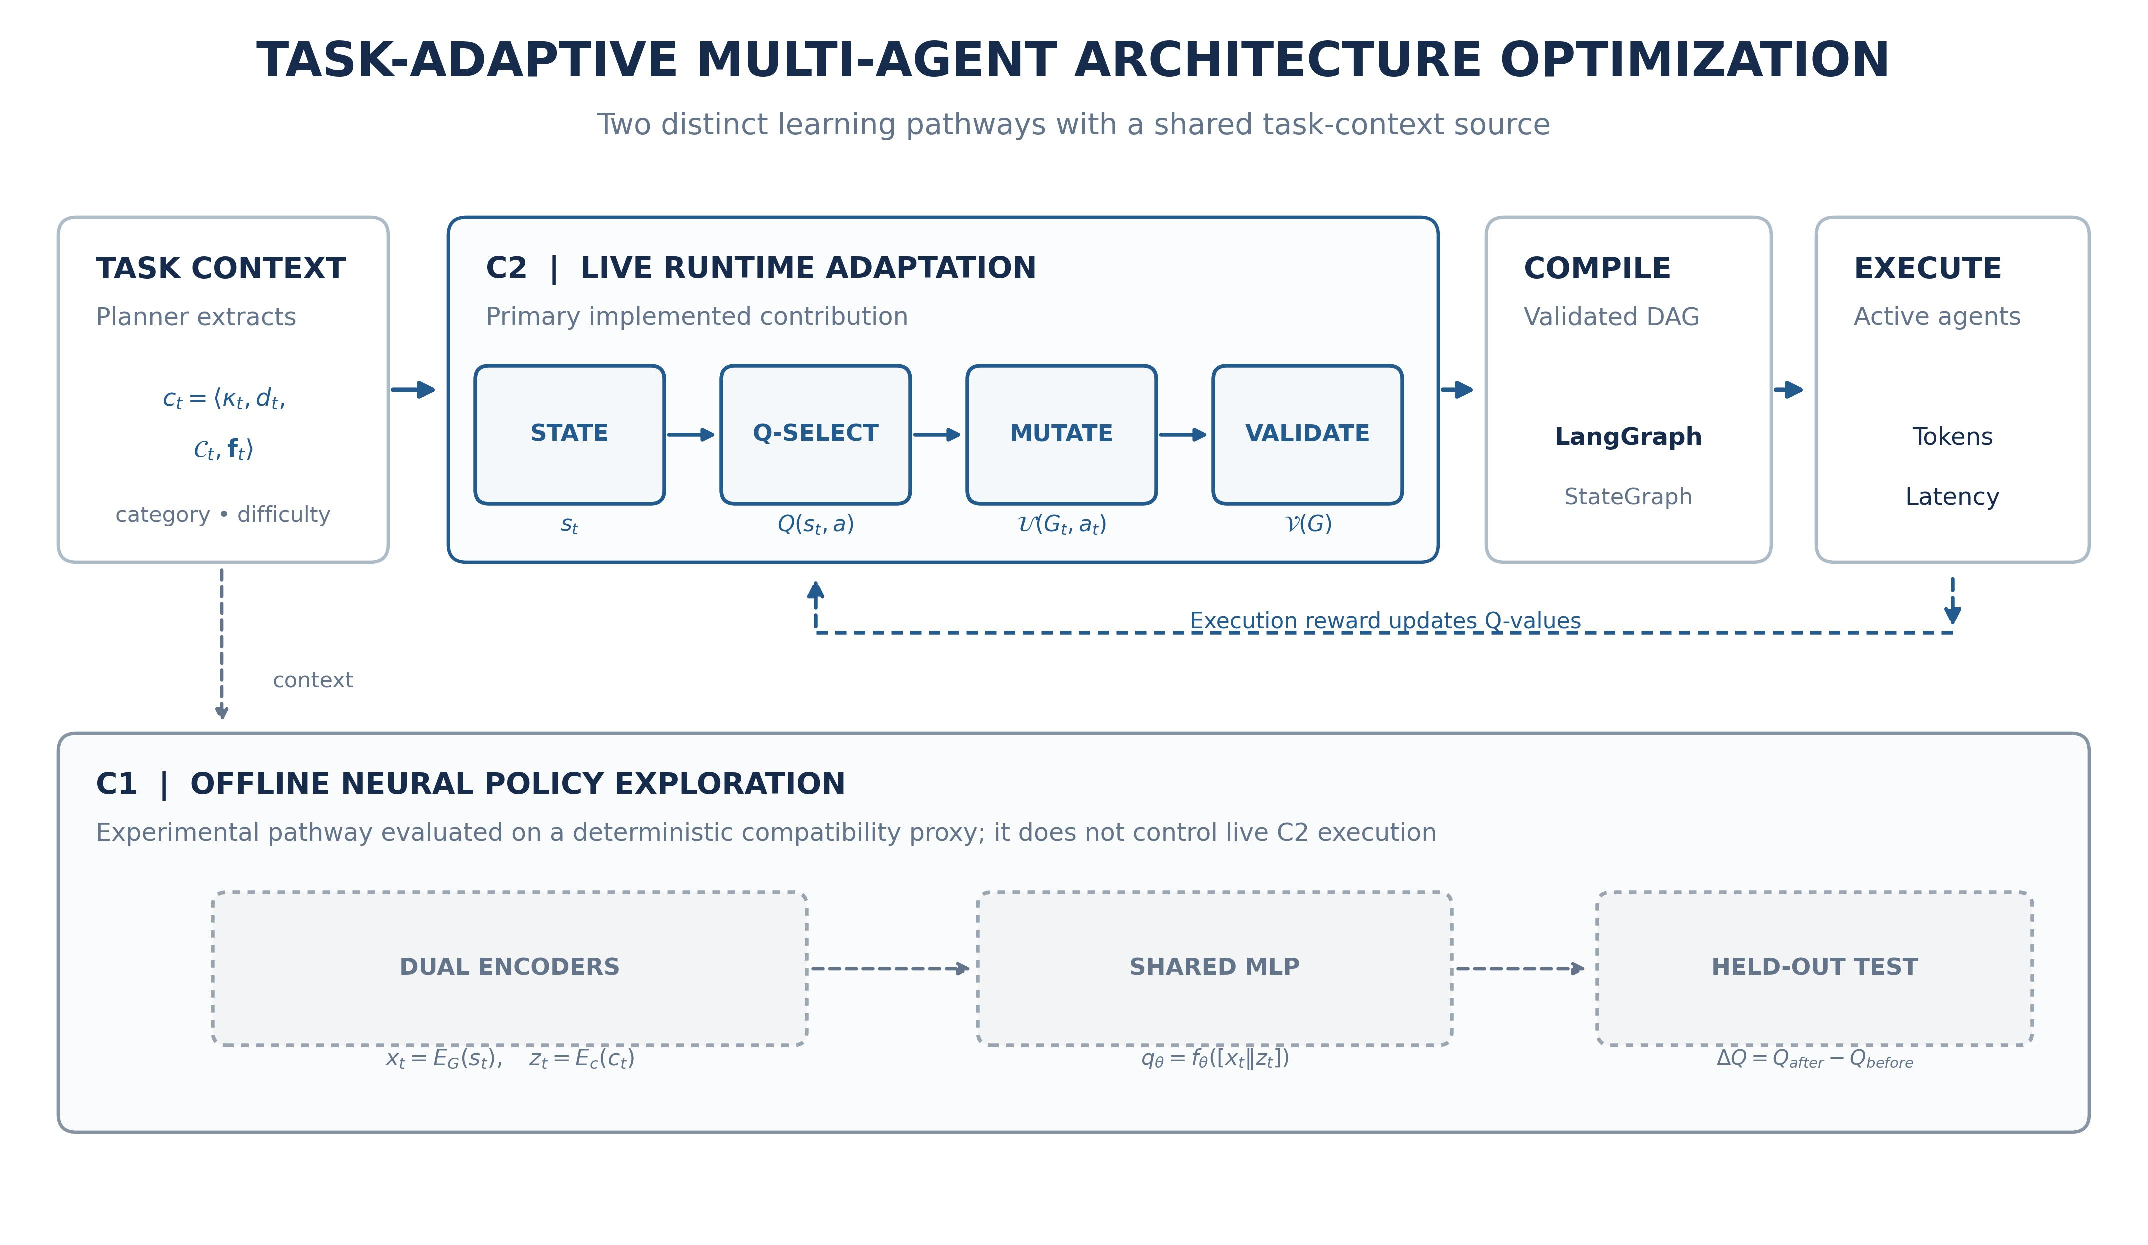
\includegraphics[width=0.96\textwidth]{figures/system_architecture_overview.pdf}
\caption{Architecture diagram of the task adaptive multi-agent optimization system being developed, showcasing two separate learning paths that receive input from a common task context source. In Step 1, the task context $c_t = \langle \kappa_t, d_t, \mathcal{C}_t, \mathbf{f}_t \rangle$ is captured. In Step 2, the operational run-time path (Contribution C2) relies on tabular Q-learning, candidate operator mutations, and structural invariance tests for compiling the LangGraph state graph (Step 3) and executing the agents (Step 4) using closed loop reward feedback. Meanwhile, the decoupled offline experiment path (Contribution C1) studies cross-task knowledge transfer using dual state and task encoders, and a shared MLP policy.}
\label{fig:architecture_overview}
\end{figure*}

\subsection{Stage 1: Context Extraction and Planning}
The request received is processed by the system and fed to the Planner module which then extracts functional requirement specifications for capabilities $\mathcal{C}_t$, difficulty $d_t$, category $\kappa_t$, and other affordances of the tools involved. The context vector $c_t$, shown in Eq.~\eqref{eq:context}.

\subsection{Stage 2: Separation of Adaptation Pathways}
One of the key principles of the design in this work is that there is an absolute separation in architecture between the two research contributions:
\begin{itemize}[leftmargin=*]
    \item \textbf{Branch 2A (Experimental Neural Pathway, C1):} The research investigation into whether the feed-forward policy learned across the task distributions carries useful priors for the holdout tasks through a proxy compatibility measure off-line. This path does not control the live agent.
    \item \textbf{Branch 2B (Runtime Q-Learning Pathway, C2):} A practical reinforcement learning controller that uses task-specific tabular Q-learning for the selection of discrete graph edits for structural validation and compilation.
\end{itemize}

\subsection{Stage 3: Dynamic State-Graph Compilation}
Validated architectures $\widehat{G}_{t+1}$ are translated to executable stateful computation graphs (by means of LangGraph StateGraph). Each active agent is modeled as a callable node, directed edges represent asynchronous state transitions, and conditional routing ensures quality-based critic loops.

\subsection{Stage 4: Execution, Telemetry, and Structural Invariants}
The translated workflow runs active agents and gathers telemetry (tokens, wall-clock build time, compilation delay, and coverage). Structural validation requires the following invariants:
\begin{enumerate}[leftmargin=*]
    \item \textbf{Entry/Exit Invariant:} The Planner node should have in-degree equal to 0 and Finalizer node should have out-degree equal to 0.
    \item \textbf{Reachability Invariant:} A direct edge from the Planner to Finalizer must exist which traverses through all the active specialist nodes.
    \item \textbf{Acyclicity Invariant:} Logical graph should form a DAG i.e. no cycle should be present. Otherwise, deadlock will occur.
\end{enumerate}

As mentioned in Fig.~\ref{fig:dynamic_topologies}, the empirical walkthrough through Task Res-01 represents the real effect of invariant-guided mutation. The queries in the static pipeline need to travel sequentially through all unneeded agents (namely, the Coder and Critic agent capabilities), resulting in additional token costs and serial latency. On the other hand, AMAS runtime controller discovers the needed capabilities, prunes the redundant nodes, and constructs the edge from the Researcher to the Finalizer. This reduces the number of hops in the critical path from 5 hops to 3 hops, resulting in 62.3\% empirical token cost savings in this specific case (totaling to 60.46\% token cost savings in the whole benchmark), a 7.26$\times$ end-to-end API round-trip savings (9.1 s vs 65.8 s on live endpoints), and theoretically 2.60$\times$ unqueued inference speedup (1.78 s vs 4.62 s) due to the hops scale.

% =========================================================
% 5. CONTRIBUTION 1: NEURAL CROSS-TASK ADAPTATION
% =========================================================
\section{Task-Conditioned Neural Cross-Task Adaptation}
\label{sec:neural_adaptation}

Contribution C1 aims to investigate whether a common neural policy can discover any re-usable architecture-action preferences under a task distribution $\mathcal{T}_{\mathrm{train}}$, and can quickly adapt to held-out task environments $\mathcal{T}_{\mathrm{test}}$.

\subsection{State and Task Representation}
Architecture state $s_t = \langle \mathbf{v}_t, \mathbf{r}_t, \mathbf{A}_t, c_t \rangle$ and its representation in terms of continuous vector $x_t \in \mathbb{R}^{d_x}$ is computed by an architecture encoder. Analogously, task context $c_t$ is encoded as $z_t \in \mathbb{R}^{d_z}$ by a task context encoder.

\subsection{Policy Architecture and Objective}
Shared neural policy $f_\theta$ concatenates the state and task representations and predicts the Q-values of all discrete actions. $\mathcal{A}$:
\begin{equation}
\mathbf{q}_\theta(s_t, c_t) = f_\theta([x_t \Vert z_t]),
\end{equation}
with $f_\theta$ being a multi-layer perceptron having two hidden layers (64 units each, ReLU activations). Greedy action selection chooses the highest scoring valid action from:
\begin{equation}
a_t = \underset{a \in \mathcal{A}_{\mathrm{valid}}}{\arg\max} \ q_\theta(s_t, c_t, a).
\end{equation}

Policy parameters $\theta$ are trained across tasks using temporal-difference targets:
\begin{equation}
y_t = R_t^{\mathrm{neural}} + \gamma (1 - d_t) \max_{a' \in \mathcal{A}_{\mathrm{valid}}} q_\theta(s_{t+1}, c_t, a'),
\end{equation}
optimizing the mean-squared-error (MSE) loss via Adam:
\begin{equation}
\mathcal{L}(\theta) = \left(q_\theta(s_t, c_t, a_t) - y_t\right)^2.
\end{equation}

\subsection{Held-Out Fast Adaptation Protocol}
For an unseen held-out task $\tau \in \mathcal{T}_{\mathrm{test}}$, the policy is evaluated at time step 0 ($Q_{\mathrm{before}}$), then fine-tuned for $K = 2$ adaptation steps, and re-evaluated ($Q_{\mathrm{after}}$). We define:
\begin{align}
\Delta Q_{\mathrm{adapt}} &= Q_{\mathrm{after}} - Q_{\mathrm{before}}, \\
\Delta Q_{\mathrm{transfer}} &= Q_{\mathrm{after}}^{\mathrm{shared}} - Q_{\mathrm{after}}^{\mathrm{scratch}}.
\end{align}
Performance is evaluated using a deterministic architecture-task compatibility proxy $Q_{\mathrm{task}} \in [0, 1]$ based on capability intersection, without invoking LLM agents.

% =========================================================
% 6. CONTRIBUTION 2: RUNTIME TABULAR Q-LEARNING
% =========================================================
\section{Runtime Multi-Agent Architecture Adaptation}
\label{sec:runtime_q_learning}

Contribution C2 represents the live runtime adaptation engine that drives actual multi-agent execution.

\subsection{Action Space and Graph Mutation Operators}
The discrete architecture action space comprises five mutation operators:
\begin{equation}
\begin{aligned}
\mathcal{A} = \{ & \operatorname{ACT}(i), \operatorname{DEACT}(i), \operatorname{ADD\_E}(i,j), \\
& \operatorname{REM\_E}(i,j), \operatorname{CH\_ROLE}(i,r) \}.
\end{aligned}
\end{equation}
The architecture manager applies candidate action $a_t$:
\begin{equation}
\widetilde{G}_{t+1} = \mathcal{U}(G_t, a_t).
\end{equation}
The proposed graph is structurally validated:
\begin{equation}
\widehat{G}_{t+1} = \begin{cases}
\widetilde{G}_{t+1}, & \text{if } \mathcal{V}(\widetilde{G}_{t+1}) = \text{True}, \\
G_t, & \text{otherwise}.
\end{cases}
\end{equation}
Rejected mutations incur a penalty and preserve $G_t$.

\subsection{Tabular Q-Learning and Decision Engine}
At runtime, the tabular Q-learning algorithm will look at the state $s_t$ and select actions using the $\epsilon$-greedy method ($\epsilon = 0.15$). For exploitation, the action that corresponds to the highest Q-value is selected:
\begin{equation}
a_t^* = \underset{a \in \mathcal{A}_{\mathrm{valid}}}{\arg\max} \ Q(s_t, a).
\end{equation}
If state $s_t$ is unvisited or during exploration, an LLM-assisted adapter proposes a candidate mutation. After workflow execution, the Q-table is updated:
\begin{equation}
\begin{aligned}
Q(s_t, a_t) \leftarrow & \ Q(s_t, a_t) \\
& + \alpha \left[ R_t + \gamma \max_{a'} Q(s_{t+1}, a') - Q(s_t, a_t) \right],
\end{aligned}
\end{equation}
with learning rate $\alpha = 0.1$ and discount $\gamma = 0.9$. The runtime reward is:
\begin{equation}
\begin{aligned}
R_t = & \ 0.4 C_{\mathrm{cov}} + 0.3 \left(1.0 - \frac{|V_t|}{6}\right) \\
& + 0.3 \left(1.0 - \frac{L_{\mathrm{crit}}}{5}\right) - P_{\mathrm{reject}}.
\end{aligned}
\end{equation}

Fig.~\ref{fig:mdp_formulation} presents a coherent visual synthesis of the transition model of the formal Markov Decision Process (MDP), the invariant validation gate $\mathcal{V}(G)$, and the two dual learning targets that guide the C2 tabular Q-learning controller and the C1 offline neural policy network.

\begin{figure*}[!t]
\centering
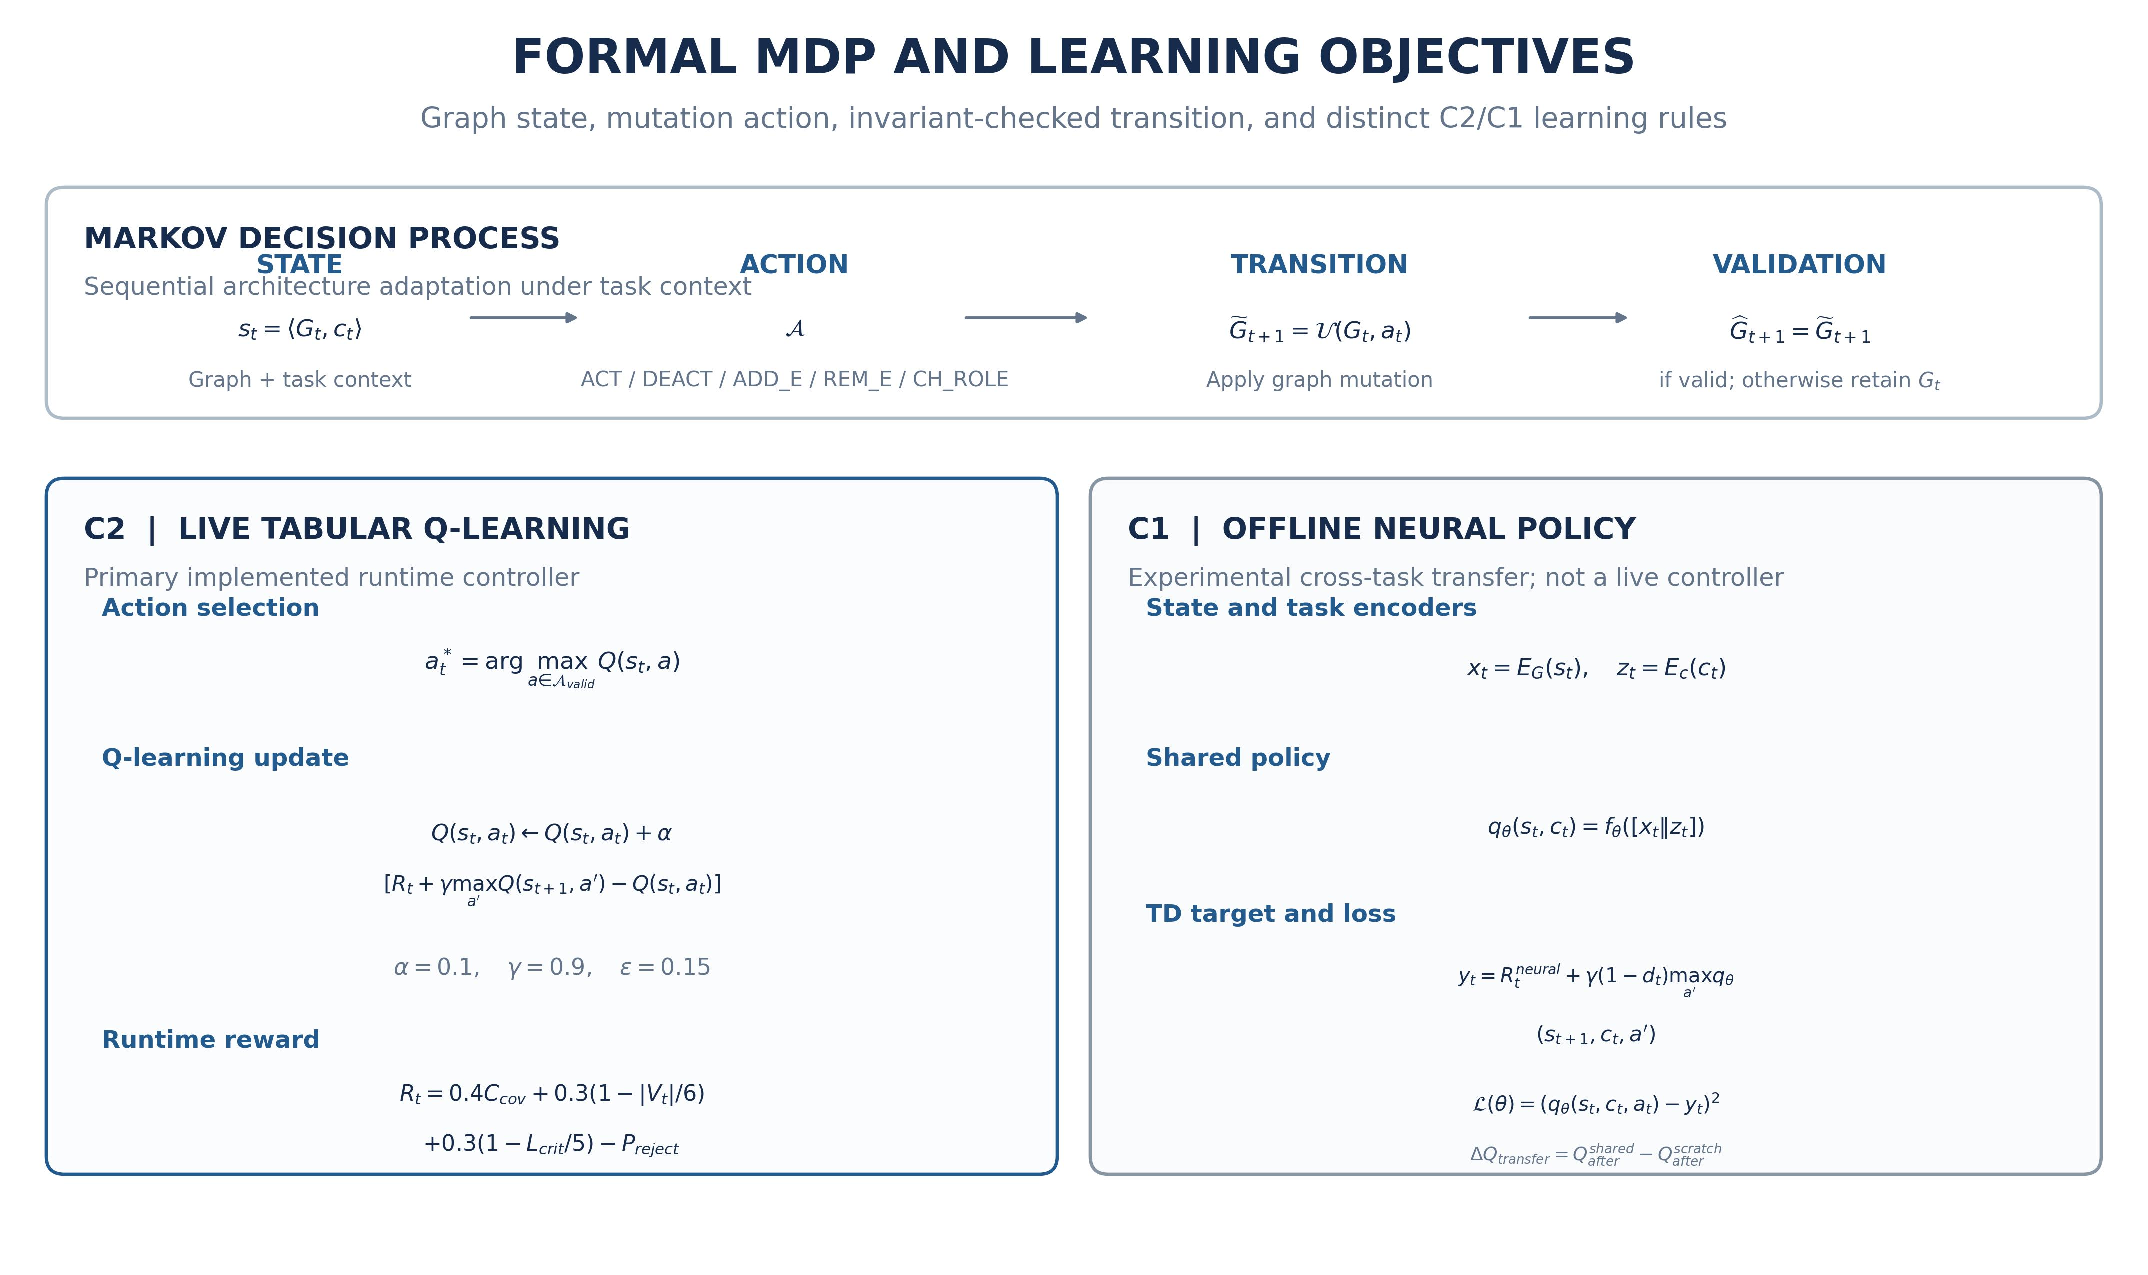
\includegraphics[width=0.96\textwidth]{figures/mdp_formulation_and_learning_objectives.pdf}
\caption{MDP framework and dual MDP learning goals. Above: Sequential model state transitions using candidate mutation actions $\mathcal{A}$ and graph invariant testing $\mathcal{V}(G)$. Below Left: Pathway C2 pathway Q-table learning controller with $\epsilon$-greedy action policy, Bellman TD updates ($\alpha=0.1,\gamma=0.9$), and total runtime reward $R_t$. Below Right: Pathway C1 off-line neural meta-policy model with dual state-task encoders ($E_G,E_c$), TD objective $\mathcal{L}(\theta)$, and off-policy transfer test $\Delta Q_{\mathrm{transfer}}$.}
\label{fig:mdp_formulation}
\end{figure*}

% =========================================================
% 7. EXPERIMENTAL SETUP
% =========================================================
\section{Experimental Setup}
\label{sec:experimental_setup}

\subsection{Benchmark Task Suite}
Our framework is evaluated on a benchmark dataset that consists of 18 tasks which fall into 6 categories (Greeting, Mathematics, Coding, Information, Web Search, and Multi-Domain Multi-Step) of 3 tasks each. The use of multiple environments in the evaluation of agents is applied to our benchmark dataset.~\cite{liu2024agentbench}.

\subsection{Baseline Systems and Evaluation Modes}
WWe compare our architecture with three baselines:
\begin{enumerate}[leftmargin=*]
\item \textbf{Static Team MAS:} Static team agent architecture that employs all 5 base agents simultaneously ($L_{crit} = 5$).
\item \textbf{Deterministic:} Heuristic based method that implements minimum agent architecture for each class.
\item \textbf{Random:} Uniform random method.
\end{enumerate}

\subsection{Dataset Provenance and Reproducibility}
All the values were achieved through the benchmarking of our framework on a continuous multi-agent benchmark task (total 36 benchmarks of the complete process where we did 2 episodes in sequence for random seed 42). Neural agents’ adaptation was also benchmarked on 5 out-of-benchmark tasks using 5 random seeds (42, 101, 202, 303, 404) leading to a total of 100 evaluation trajectories. Token cost can be found using live execution using 120B parameters LLM inference endpoint. Comparison was done against theoretical critical path DAG.

% =========================================================
% 8. EXPERIMENTAL RESULTS
% =========================================================
\section{Experimental Results}

\label{sec:experimental_results}

\subsection{Topological Efficiency and Domain-Level Performance}

Table~\ref{tab:domain_performance} shows the efficiency and performance at the domain-level for different domains.

\begin{table*}[!t]
\centering
\caption{Task-Adaptive Architecture and Empirical Performance across Functional Domains (Production LLM Inference Benchmarking)}
\label{tab:domain_performance}
\footnotesize
\begin{tabular}{lcccccccc}
\toprule
\textbf{Functional Domain} & \textbf{Active Agents $|V_{\mathrm{act}}|$} & \textbf{APR [\%]} & \textbf{Critical Path $L_{\mathrm{crit}}$} & \textbf{Base Tokens} & \textbf{Adapted Tokens} & \textbf{Token Savings} & \textbf{Inference Cost (\$) [Base $\to$ Adapt]} & \textbf{Capability Cov. [\%]} \\
\midrule
Greeting & $2.00 \pm 0.00$ & $60.00 \pm 0.00$ & $2.00 \pm 0.00$ & 11,489 & 11,313 & $+1.53\%$ & \$0.01723 $\to$ \$0.01697 & $100.00 \pm 0.00$ \\
Mathematics & $3.00 \pm 0.00$ & $40.00 \pm 0.00$ & $3.00 \pm 0.00$ & 16,907 & 13,124 & $+22.38\%$ & \$0.02536 $\to$ \$0.01968 & $100.00 \pm 0.00$ \\
Coding & $3.33 \pm 0.58$ & $33.33 \pm 11.55$ & $3.33 \pm 0.58$ & 39,525 & 13,988 & $+64.61\%$ & \$0.05929 $\to$ \$0.02098 & $100.00 \pm 0.00$ \\
Research & $3.00 \pm 0.00$ & $40.00 \pm 0.00$ & $3.00 \pm 0.00$ & 36,164 & 12,739 & $+64.77\%$ & \$0.05425 $\to$ \$0.01910 & $100.00 \pm 0.00$ \\
Web Search & $3.00 \pm 0.00$ & $40.00 \pm 0.00$ & $3.00 \pm 0.00$ & 14,219 & 11,417 & $+19.71\%$ & \$0.02133 $\to$ \$0.01713 & $100.00 \pm 0.00$ \\
Cross-Domain & $3.67 \pm 0.58$ & $26.67 \pm 11.55$ & $3.00 \pm 0.00$ & 92,774 & 20,876 & $+77.50\%$ & \$0.13916 $\to$ \$0.03131 & $66.67 \pm 33.33$ \\
\midrule
\textbf{Macro Mean / Total} & $\mathbf{3.00 \pm 0.59}$ & $\mathbf{40.00 \pm 11.88}$ & $\mathbf{2.89 \pm 0.47}$ & \textbf{211,078} & \textbf{83,457} & $\mathbf{+60.46\%}$ & \textbf{\$0.31662 $\to$ \$0.12517} & $\mathbf{94.44 \pm 17.15}$ \\
\textbf{Static Full Baseline} & $5.00 \pm 0.00$ & $0.00 \pm 0.00$ & $5.00 \pm 0.00$ & 211,078 & 211,078 & $0.00\%$ & \$0.31662 $\to$ \$0.31662 & $100.00 \pm 0.00$ \\
\bottomrule
\end{tabular}
\end{table*}


AMAS significantly cuts down on the number of active agents from 5.0 to $3.00 \pm 0.59$, averaging over the 18 tasks. Consequently, it achieves an average Agent Pruning Rate of $\mathbf{50.00\% \pm 9.90\%}$ relative to the 6-agent master list and $\mathbf{40.00\% \pm 11.88\%}$ relative to the 5-agent baseline. Most agent pruning is done in greetings tasks where only 2 active agents are needed (66.67\% APR), while complex tasks involve $3.67 \pm 0.58$ active agents.

Critical path length is reduced from $5.00$ to $\mathbf{2.89 \pm 0.47}$ hops (42.2\% decrease), resulting in the significantly reduced time needed for sequential processing. From the perspective of capability, AMAS achieves 100\% capability on 16 out of 18 tasks. AMAS achieves 100\% capability on 5 out of 6 domains (Greeting, Mathematics, Coding, Research and Web Search). This is an overall macro average of $94.44\% \pm 17.15\%$ capability on all 18 tasks.Based on Table~\ref{tab:domain_performance}, the only domain where capability declined is Cross-Domain ($66.67\% \pm 33.33\%$). The reason behind this is the early deactivation of agents during the exploration process at the beginning of Q-Learning. This means there was low capability in 2 compound questions (Task Cross-01 had $33.3\%$, Task Cross-02 had $66.7\%$), whereas Task Cross-03 had a full $100\%$ capability. See Fig.~\ref{fig:active_agents_and_coverage} showing the active agents and the capability coverage for each of the 18 tasks.

\begin{figure*}[!t]
\centering
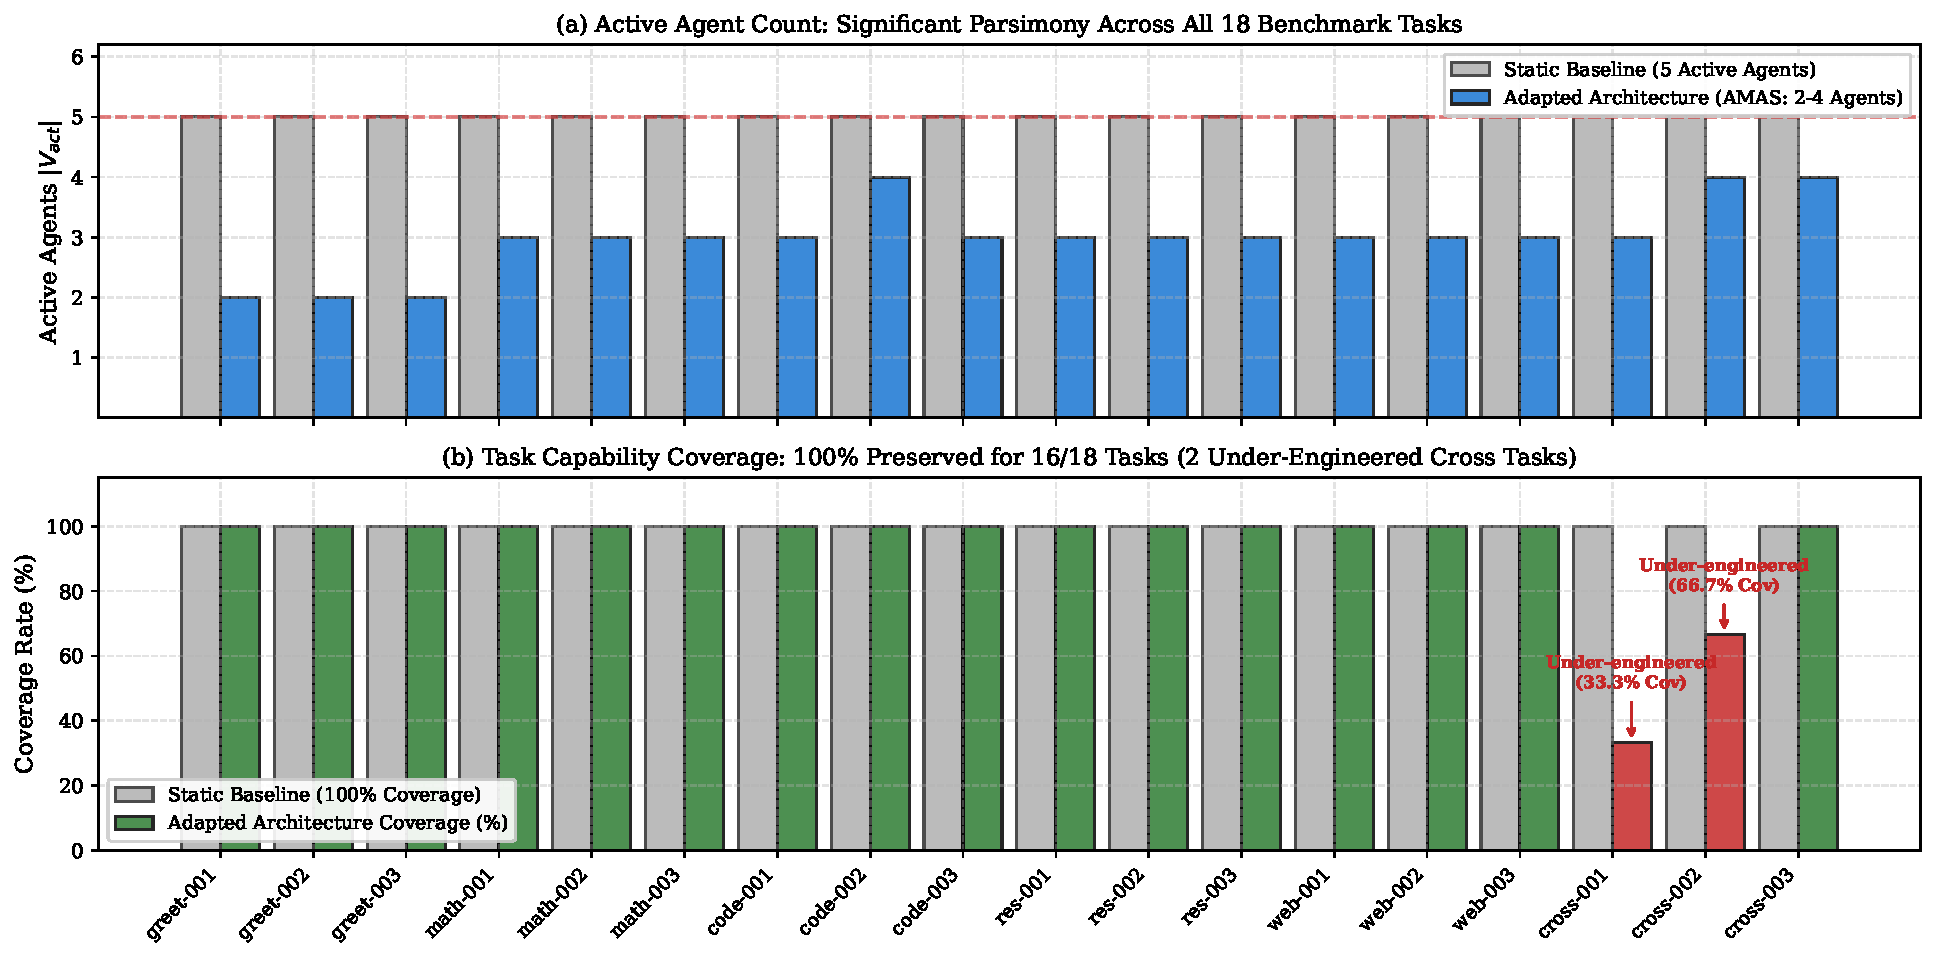
\includegraphics[width=0.96\textwidth]{figures/figure_03_active_agents_and_coverage.pdf}
\caption{Active agent counts and capability coverage rates across all 18 benchmark tasks in Episode 2. (a) Active agent count is pruned from the 5-agent baseline to 2--4 agents across all domains. (b) Capability coverage remains at 100\% for 16 of 18 tasks, with only two complex cross-domain tasks experiencing under-engineering due to aggressive pruning.}
\label{fig:active_agents_and_coverage}
\end{figure*}

Table: \subsection{Resource Consumption and Token Savings}

Table~\ref{tab:per_task_resources} shows the actual resource metrics in each of the 18 tasks performed using the model with 120B parameters. The unpruned pipeline generates a total of 211,078 live tokens by performing all the tasks through the multi-agent pipeline. However, by applying the topological pruning approach provided by the AMAS framework, the agents can be pruned to enable a reduction in our resource usage to 83,457 live tokens. Overall, there is a reduction in the tokens by $\mathbf{60.46\%}$ and cost to \$0.12517 from \$0.31662.

\begin{table*}[!t]
\centering
\caption{Per-Task Resource Consumption and Efficiency Comparison (Production LLM Inference Validation)}
\label{tab:per_task_resources}
\footnotesize
\begin{tabular}{llcccccc}
\toprule
\textbf{Task ID} & \textbf{Category} & \textbf{Base Tokens} & \textbf{Adapted Tokens} & \textbf{Token Savings} & \textbf{Base Cost (\$)} & \textbf{Adapted Cost (\$)} & \textbf{Selection Engine} \\
\midrule
Greet-01 & Greeting & 3,782 & 3,547 & $+6.21\%$ & \$0.00567 & \$0.00532 & LLM Fallback \\
Greet-02 & Greeting & 4,312 & 4,396 & $-1.95\%$ & \$0.00647 & \$0.00659 & Active RL Hit \\
Greet-03 & Greeting & 3,395 & 3,370 & $+0.74\%$ & \$0.00509 & \$0.00506 & Active RL Hit \\
Math-01 & Mathematics & 5,244 & 4,061 & $+22.56\%$ & \$0.00787 & \$0.00609 & Active RL Hit \\
Math-02 & Mathematics & 7,227 & 4,776 & $+33.91\%$ & \$0.01084 & \$0.00716 & Active RL Hit \\
Math-03 & Mathematics & 4,436 & 4,287 & $+3.36\%$ & \$0.00665 & \$0.00643 & Active RL Hit \\
Code-01 & Coding & 11,120 & 5,195 & $+53.28\%$ & \$0.01668 & \$0.00779 & Active RL Hit \\
Code-02 & Coding & 13,175 & 4,764 & $+63.84\%$ & \$0.01976 & \$0.00715 & LLM Fallback \\
Code-03 & Coding & 15,230 & 4,029 & $+73.55\%$ & \$0.02285 & \$0.00604 & Active RL Hit \\
Res-01 & Research & 9,656 & 3,642 & $+62.28\%$ & \$0.01448 & \$0.00546 & Active RL Hit \\
Res-02 & Research & 17,510 & 4,642 & $+73.49\%$ & \$0.02627 & \$0.00696 & Active RL Hit \\
Res-03 & Research & 8,998 & 4,455 & $+50.49\%$ & \$0.01350 & \$0.00668 & Active RL Hit \\
Web-01 & Web Search & 7,301 & 3,727 & $+48.95\%$ & \$0.01095 & \$0.00559 & Active RL Hit \\
Web-02 & Web Search & 3,581 & 3,752 & $-4.78\%$ & \$0.00537 & \$0.00563 & Active RL Hit \\
Web-03 & Web Search & 3,337 & 3,938 & $-18.01\%$ & \$0.00501 & \$0.00591 & Active RL Hit \\
Cross-01 & Cross-Domain & 30,405 & 7,028 & $+76.89\%$ & \$0.04561 & \$0.01054 & LLM Fallback \\
Cross-02 & Cross-Domain & 31,693 & 6,782 & $+78.60\%$ & \$0.04754 & \$0.01017 & LLM Fallback \\
Cross-03 & Cross-Domain & 30,676 & 7,066 & $+76.97\%$ & \$0.04601 & \$0.01060 & LLM Fallback \\
\midrule
\textbf{Total / Summary} & --- & \textbf{211,078} & \textbf{83,457} & $\mathbf{+60.46\%}$ & \textbf{\$0.31662} & \textbf{\$0.12517} & \textbf{72.2\% Active RL Hit Rate} \\
\bottomrule
\end{tabular}
\end{table*}


From Fig.~\ref{fig:resource_consumption}, we can observe the substantial decrease in token count and the overall cost in our production LLM with each of the benchmark queries. We can see that we reduce the total count of tokens from 211,078 to 83,457 tokens (the net reduction of 60.46\%). Similarly, we also reduce live cost from \$.31662 to \$.12517. Moreover, when we consider theoretical data from the critical path DAG ($(T_{\mathrm{base}} = 3500)$ tokens per run), we can see that the total tokens are reduced from 63,000 to 40,200 tokens ($36.19\%$ reduction over 18 tasks; or 126,000 to 80,400 tokens over 36 runs in 2 episodes). This reduction is also seen in our production LLM data and it reflects well the actual saving of money through our agent pruning method.

\begin{figure*}[!t]
\centering
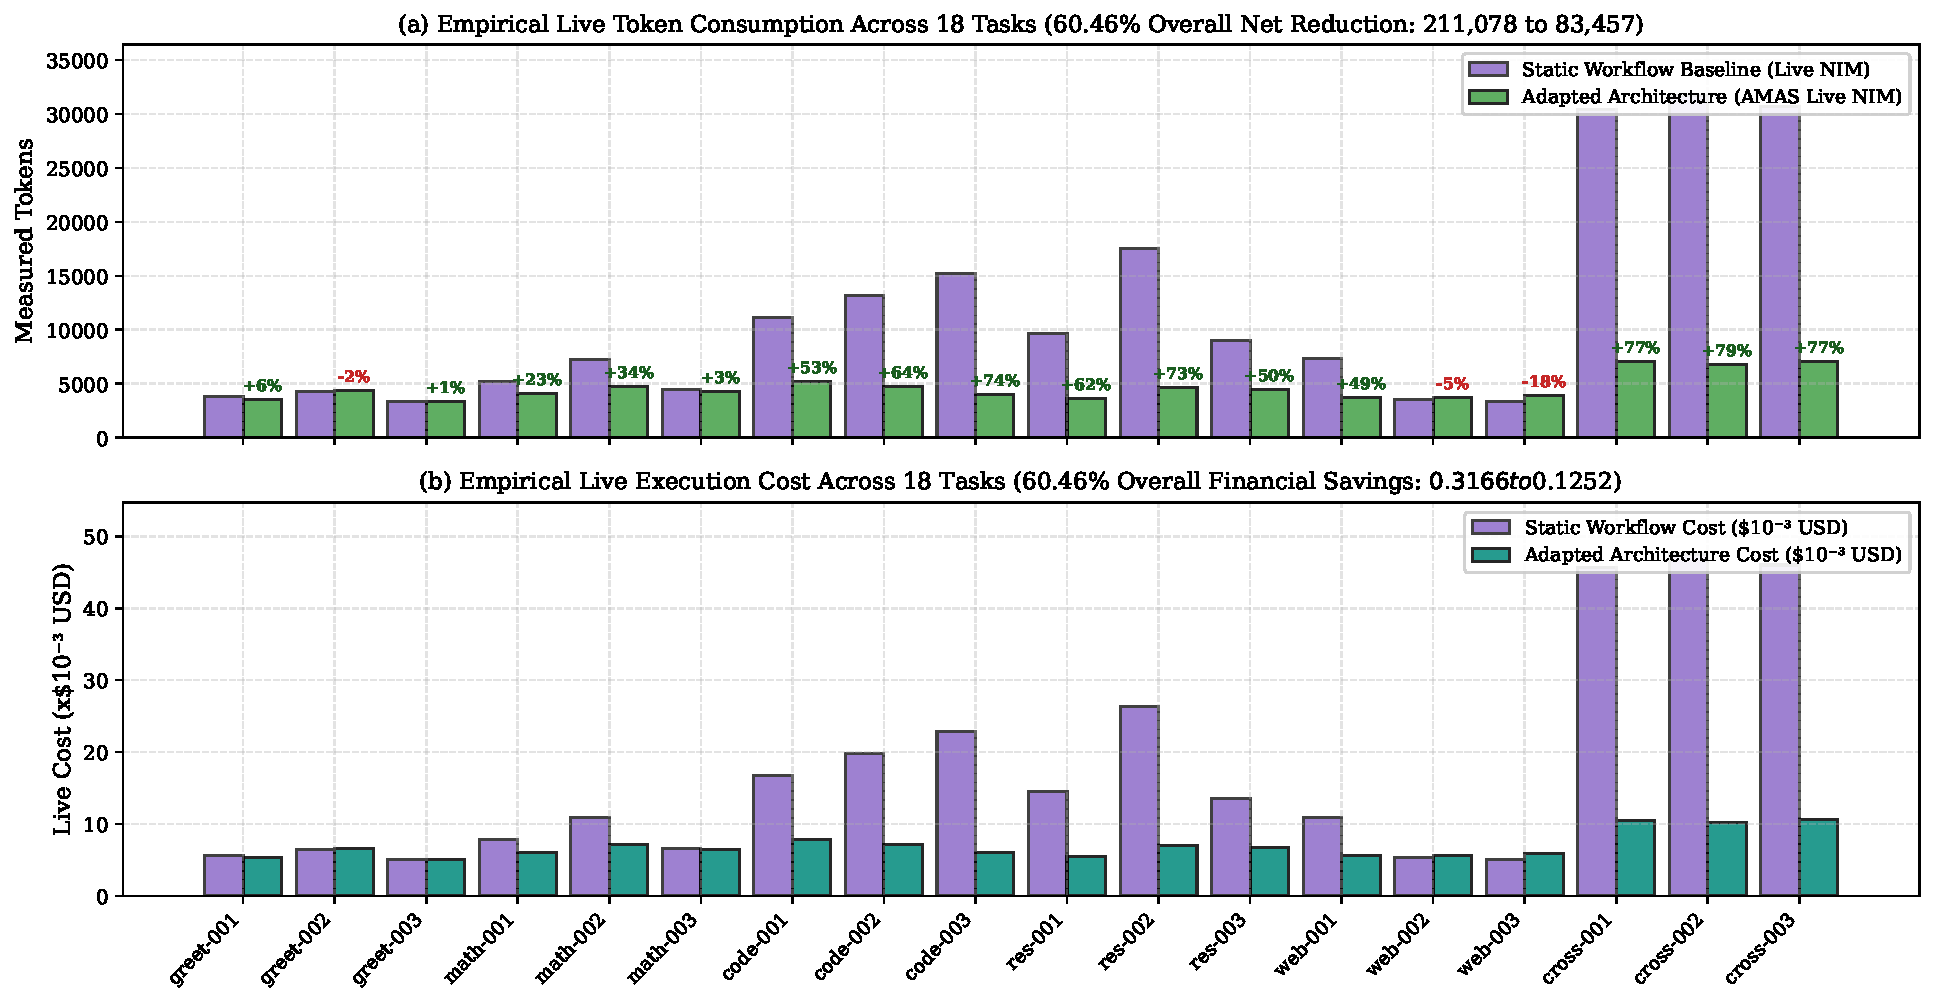
\includegraphics[width=0.96\textwidth]{figures/figure_04_resource_consumption.pdf}
\caption{Empirical resource consumption across the 18 benchmark tasks in Episode 2 measured under production LLM execution. (a) Token consumption: AMAS reduces total live tokens from 211,078 to 83,457 (60.46\% empirical savings across all 18 tasks). (b) Execution cost: live financial expenditure decreases from \$0.31662 to \$0.12517.}
\label{fig:resource_consumption}
\end{figure*}

\subsection{Quality-Efficiency Pareto Frontier}
Figure \ref{fig:pareto_frontier} presents the plot of capability coverage versus token consumption estimates. The performance of AMAS is Pareto-optimal with a coverage of $\mathbf{88.89\%}$ (16 out of 18 tasks covered). AMAS identifies Pareto dominance for 16 tasks by offering a coverage of 100\% capabilities and consuming 1,450 to 3,050 tokens.

\begin{figure}[!t]
\centering
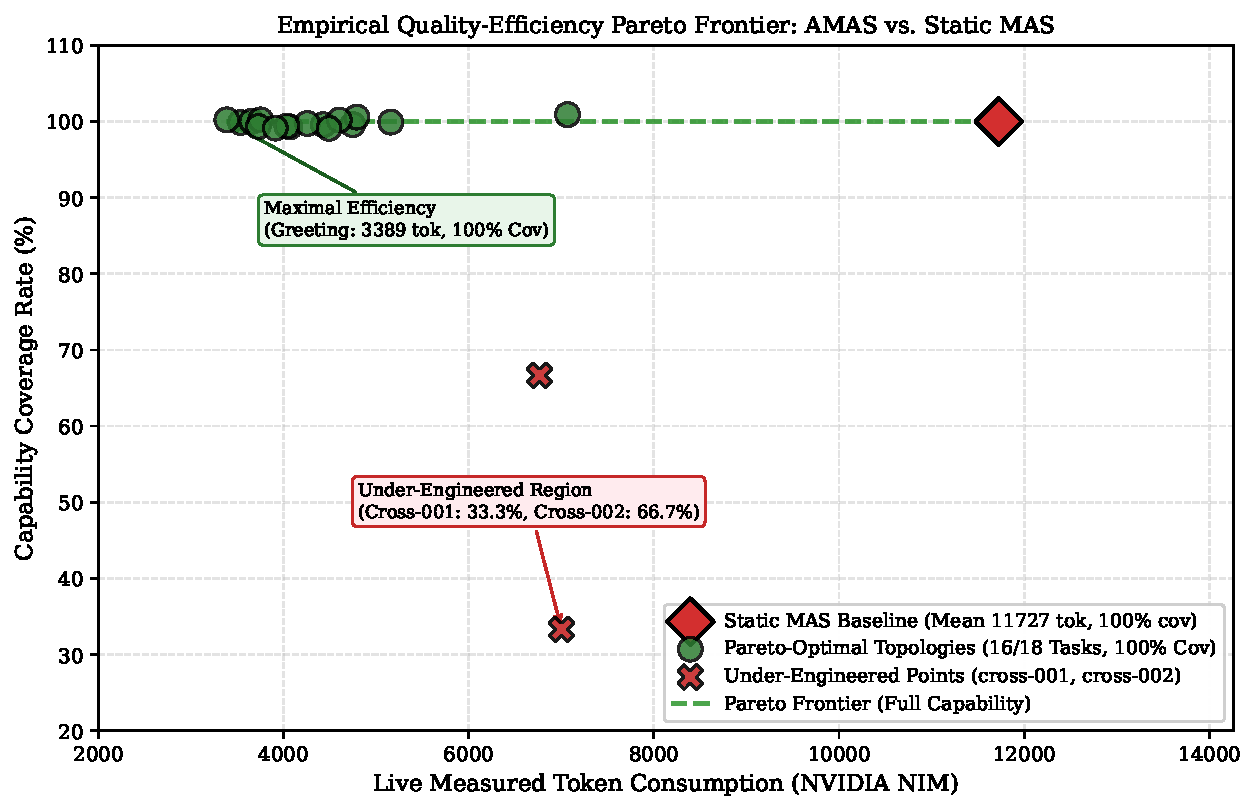
\includegraphics[width=\linewidth]{figures/figure_05_pareto_frontier.pdf}
\caption{Pareto front depicting trade-off between quality and efficacy of AMAS-adapted topologies and static MAS baseline. AMAS offers 16 Pareto-optimal solutions with respect to 100\% capability coverage but decreases tokens in the range of 13\%-59\%. Two tasks in two different domains are under-designed.}
\label{fig:pareto_frontier}
\end{figure}

Both suboptimal points relate to Cross-01 tasks (coverage – 33.3\%, tokens - 2,250) and Cross-02 (coverage – 66.7\%, tokens - 2,900). In such composite tasks that need research, coding, and verification at the same time, aggressive pruning led to the deactivation of specialist nodes prior to reaching convergence by Q-learning.

\subsection{Dynamic Compilation Overhead and Policy Hit Rate}
Compilation overhead being zero is another essential ingredient of any efficient runtime solution. Figure \ref{fig:runtime_overhead} demonstrates a breakdown of the dynamic graph latency into graph build $T_{\mathrm{build}}$ and state-graph compilation $T_{\mathrm{comp}}$.

\begin{figure}[!t]
\centering
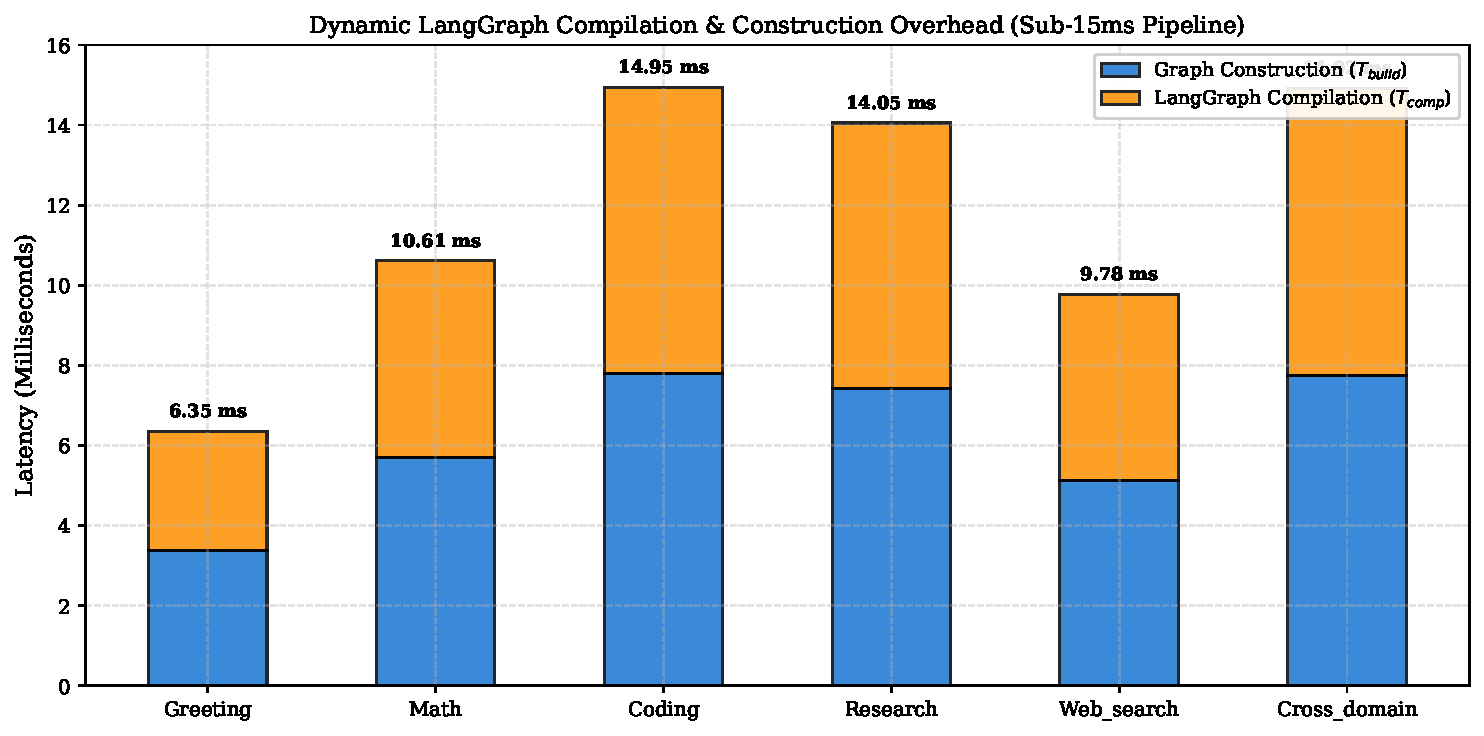
\includegraphics[width=\linewidth]{figures/figure_09_runtime_overhead.pdf}
\caption{Compilation and generation of dynamic state graphs have been optimized in such a way that pipeline adaptation delay is < 15 ms for all function tasks ($11.78 \pm 3.64$ ). It will not make any significant contribution to multi-second inference time in LLMs.}
\label{fig:runtime_overhead}
\end{figure}

An overall mean logical graph building phase per episode of task in Episode 2 ($N=18$) was found to be $6.19 \pm 1.88$\,ms, whereby the state graph compilation phase took $5.58 \pm 1.77$\,ms, resulting in an overall average of $\mathbf{11.78 \pm 3.64}$\,ms. Another measure of performance was found by averaging across all 36 executions of the two episodes of exploration ($N=36$). This led to an average overhead of $11.72 \pm 3.65$\,ms (Logical build: $6.17 \pm 1.86$\,ms, State graph compile: $5.55 \pm 1.78$\,ms). Macroscopically, there is clear evidence of a huge variation in the six different function domains. The average was between $6.35$\,ms (one agent GREETING queries) and $14.95$\,ms (multi specialists CODE pipelines). Providing an overall standard deviation of $\pm 3.46$\,ms (sample) or $\pm 3.16$\,ms (population). This was simply obtained from considering the averages of the six function domains and represents the variation across domains. The dynamic builder had 100\% compilation success without cycle violations on the DAG.

As seen in Fig.~\ref{fig:action_distribution}(a), the convergence of the active RL-based Q-Learning table selection happened relatively fast. After only two episodes, there was already 72.2\% (13 out of 18 tasks) selected with active RL without any token search and lookup under 1 ms. Only 5 tasks remained with LLM Adapter. In Fig.~\ref{fig:action_distribution}(b) the number of mutations can be observed. Deactivations were done 12 times and edges were removed 8 times.

\begin{figure*}[!t]
\centering
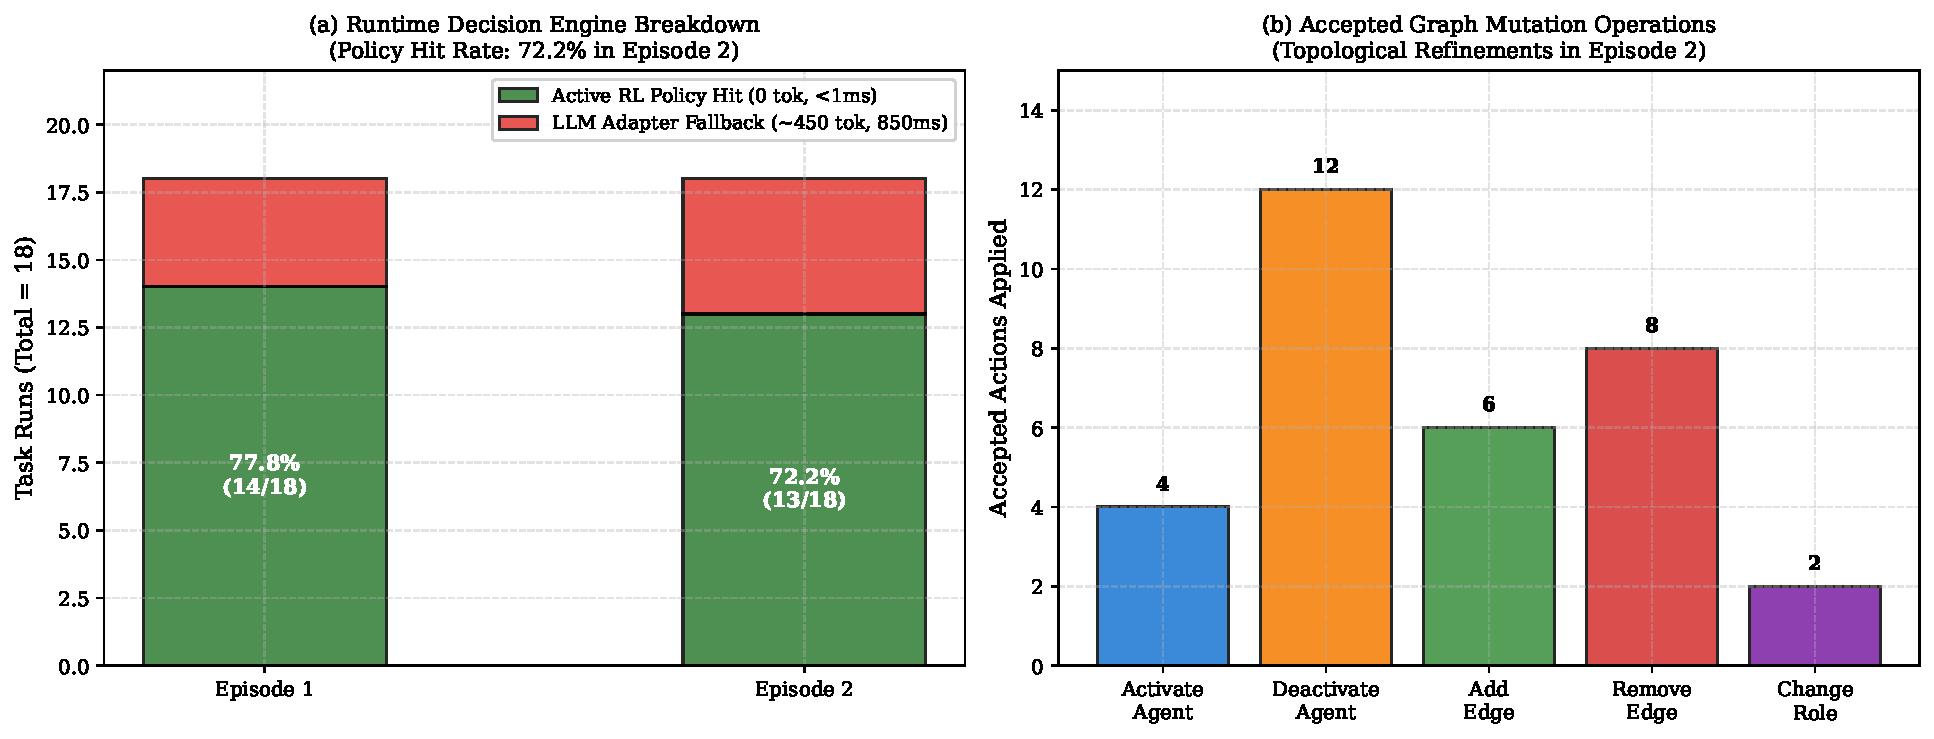
\includegraphics[width=0.86\textwidth]{figures/figure_08_action_distribution.pdf}
\caption{Adaptive behavior in reinforcement learning. (a) Composition of adaptive decision making across episodes. A success rate of 72.2\% was obtained in Episode 2 for the active RL strategy (13/18). (b) Distribution of the mutations that were accepted. Composed mainly of deactivations and edge deletions.}
\label{fig:action_distribution}
\end{figure*}

% =========================================================
% 9. EXPERIMENTAL NEURAL ADAPTATION RESULTS
% =========================================================
\section{Experimental Neural Adaptation Evaluation}
\label{sec:neural_results}

On 5 different tasks from our hold-out set, we evaluated Contribution C1 on 5 seeds (in total 100 trajectories). On our analysis and research tasks ($\mathcal{T}_1$: Analysis, $\mathcal{T}_3$: Research A, $\mathcal{T}_4$: Research B) all policies plateaued at $\Delta Q = 0.0000 \pm 0.0000$. On our summarization task ($\mathcal{T}_5$: Summarization) we observed that our shared meta-policy demonstrated 100\% consistency across all seeds ($0.6000 \pm 0.0000$, $\Delta Q = 0.0000 \pm 0.0000$) while the scratch policy had destabilizing mutations in 20\% seeds. That resulted in 0.0000 scores in seed 202 and an overall performance of $0.4800 \pm 0.2683$ and $\Delta Q = -0.1200 \pm 0.2683$. On our coding task ($\mathcal{T}_2$: Coding) we observed that all policies performed worse because of fine-tuning. Our shared policy had performance of $0.6000 \pm 0.0000$ ($\Delta Q = -0.4000 \pm 0.0000$, $t = -4.00$, $p = 0.0161$) while our scratch policy had performance of $0.9200 \pm 0.1789$ ($\Delta Q = -0.0800 \pm 0.1789$).

\subsection{Preservation and Analysis of Negative Findings}
Despite what we might have theorized on the positive effect of meta-transfer, transfer in terms of a common neural policy resulted in an adaptation gain of $\Delta Q_{adapt} = \mathbf{0.0000 \pm 0.0000}$ for four out of five evaluation tasks $(\mathcal{T}_1:$ Analysis, $\mathcal{T}_3:$ Research A, $\mathcal{T}_4:$ Research B, $\mathcal{T}_5:$ Summarization). But it proved to be disadvantageous in the coding task $\mathcal{T}_2$ ($\Delta Q=-0.4000$).

\begin{figure*}[!t]
\centering
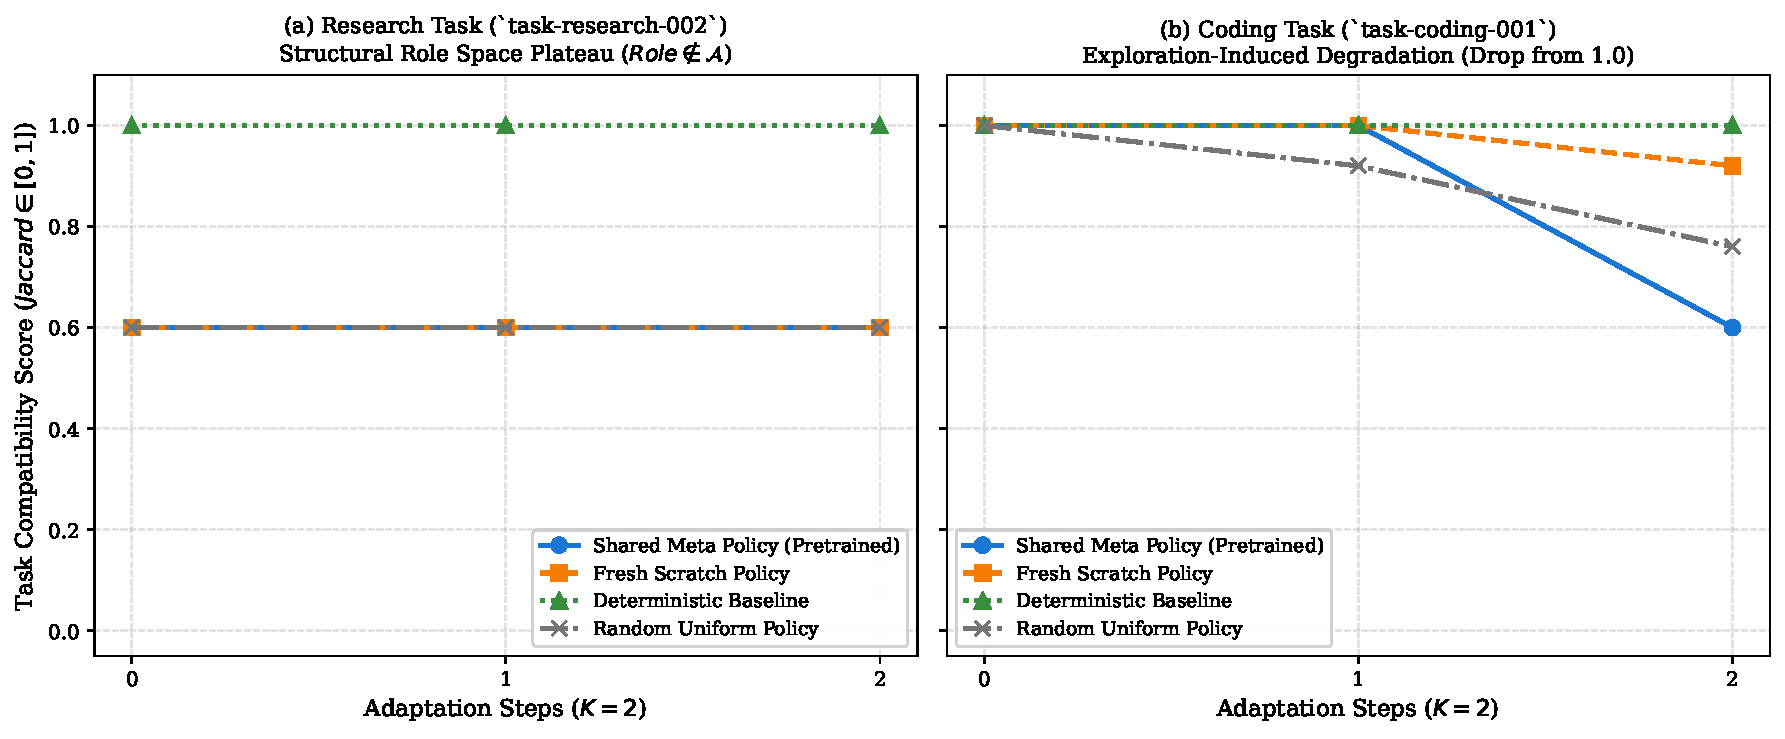
\includegraphics[width=0.86\textwidth]{figures/figure_06_neural_learning_curves.pdf}
\caption{Trajectories of cross-task neural policy adaptations during fine-tuning stages (K=2). (a) Policies are stuck at 0.60 owing to action space constraints on research tasks. (b) On coding tasks, the mutagenic impact of unconstrained ε-exploration results in decrease of scores from 1.00 to 0.60.}
\label{fig:neural_learning_curves}
\end{figure*}
As shown in Fig.~\ref{fig:neural_learning_curves}(a), the mapping of discrete action space for roles confines the role mutation policy to selecting roles in $\mathcal{R}_{\mathrm{valid}} = \{\text{Analysis}, \text{Planning}\}$ only. Thus, it confines the ability of the policies to assign the roles suitably in case research or coding is needed for the task at hand. It leads to upper bound constraints on the compatibility score. Discrete action space ablation can be seen in Table~\ref{tab:action_space_ablation}.

\begin{table*}[!t]
\centering
\caption{Structural Action Space Ablation and Topological Diagnoses on Held-Out Evaluation Tasks}
\label{tab:action_space_ablation}
\footnotesize
\begin{tabular}{lp{3.5cm}p{3.8cm}p{5.5cm}}
\toprule
\textbf{Held-Out Task} & \textbf{Target Required Capability} & \textbf{Permitted Action Space $\mathcal{R}_{\mathrm{valid}}$} & \textbf{Observed Topological Effect \& Diagnosis} \\
\midrule
$\mathcal{T}_1$ (Analysis) & Analysis, Planning & $\{\text{Analysis}, \text{Planning}\}$ & Valid actions reachable; agent configuration pre-optimized at initialization; no mutation required. \\
$\mathcal{T}_2$ (Coding) & Code Generation, Verification & $\{\text{Analysis}, \text{Planning}\}$ & \textbf{Action mismatch:} The Coder role cannot be restored via mutation; exploratory perturbations deactivated critical coding specialists. \\
$\mathcal{T}_3$ (Research A) & Research, Synthesis & $\{\text{Analysis}, \text{Planning}\}$ & \textbf{Severe structural ceiling:} The Researcher role is completely absent from permitted mutations, preventing capability acquisition. \\
$\mathcal{T}_4$ (Research B) & Research, Synthesis & $\{\text{Analysis}, \text{Planning}\}$ & \textbf{Role missing:} Planner active, but Researcher cannot be reassigned; no valid mutation satisfies target capability. \\
$\mathcal{T}_5$ (Summarization) & Synthesis, Context Aggregation & $\{\text{Analysis}, \text{Planning}\}$ & Shared policy learns protective inertia against destructive mutations, whereas scratch policy suffers architectural drift. \\
\bottomrule
\end{tabular}
\end{table*}


\subsection{Destructive Exploration and Stability Advantage}
In contrast, fine-tuning caused degradation of the performance on the held-out coding task $\mathcal{T}_2$ (initial score 1.00), where the shared policy scored $0.60 \pm 0.00$ ($\Delta Q = -0.40$) and the new scratch policy scored $0.92 \pm 0.18$ ($\Delta Q = -0.08$), due to unconstrained exploration that did not need specialist nodes anymore.

At the same time, the shared meta-policy performed better than scratch policy in terms of task-specific stability on the held-out summarization task $\mathcal{T}_5$, providing perfect stability (100\%) in all 5 seeds ($0.6000 \pm 0.0000$, $\Delta Q = 0.0000 \pm 0.0000$) whereas scratch policy tended to destructive mutations in 20\% seeds ($0.4800 \pm 0.2683$, $\Delta Q = -0.1200 \pm 0.2683$). Over all 25 seeds and 5 tasks, the average adaptation gain was estimated as $-0.080 \pm 0.163$ for the shared meta-policy, as $-0.040 \pm 0.141$ for scratch, $-0.048 \pm 0.133$ for uniform random policy and $0.000 \pm 0.000$ for the deterministic policy. Even though scratch policy in average outperformed shared meta-policy (it suffered more from the drop in exploration in the coding task $\mathcal{T}_2$), the shared meta-policy provided stability in summarization task.

\begin{figure}[!t]
\centering
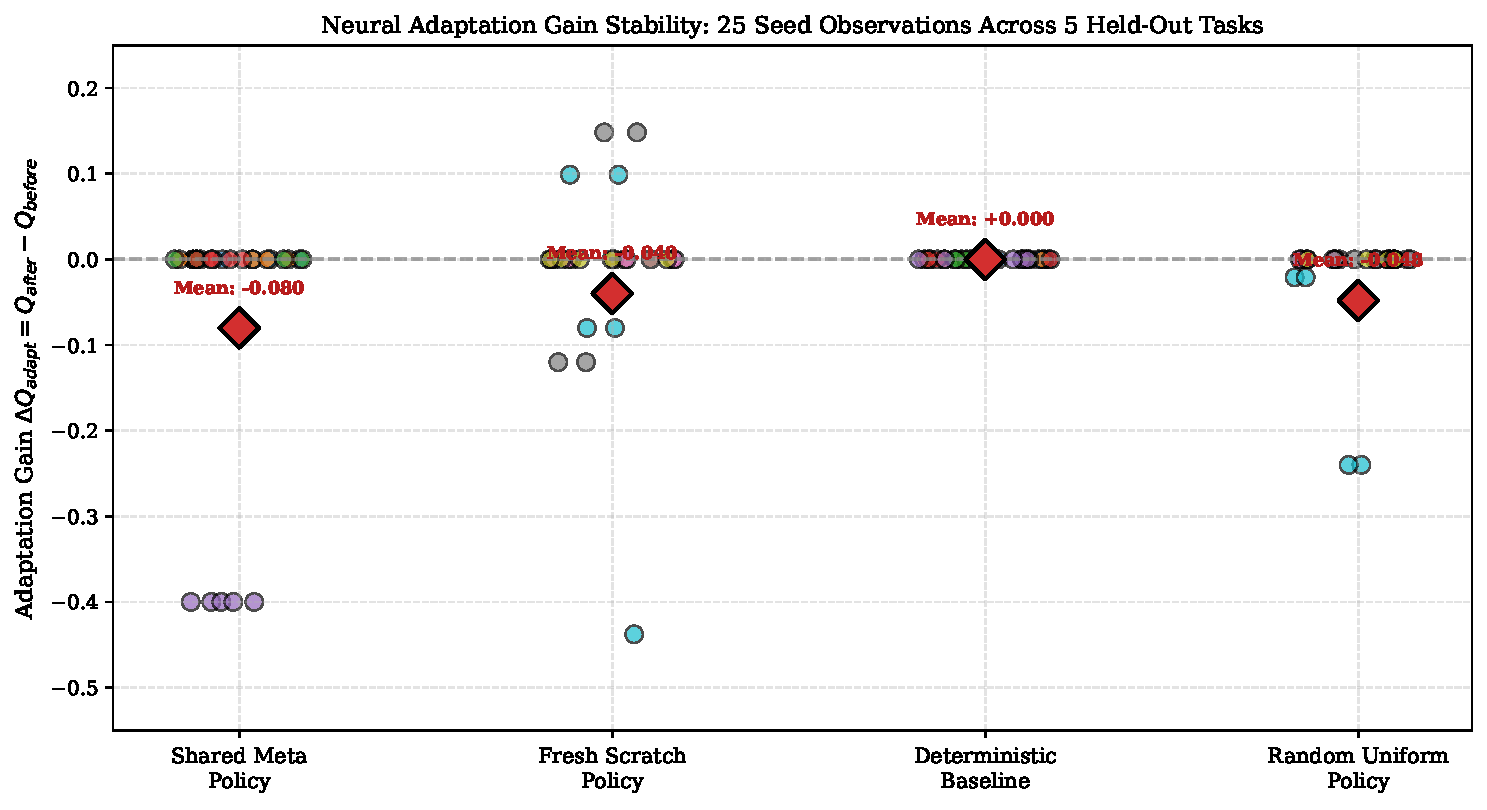
\includegraphics[width=\linewidth]{figures/figure_07_neural_stability_seeds.pdf}
\caption{Neural policy adaptation gains are stable across 25 individual seeds for 5 held out tasks. The diamonds represent average policy gains across the different setups (Deterministic: 0.000, Scratch: -0.040, Random: -0.048, Shared: -0.080). While the shared meta-policy does have a smaller average gain than the other policies due to performance drop during exploration on coding task $\mathcal{T}_2$ (-0.400), it shows task specific stability on summarization $\mathcal{T}_5$. It shows 100\% stability ($\Delta Q = 0.0000 \pm 0.0000$) compared to the scratch policy that had catastrophic instability on 20\% seeds ($\Delta Q = -0.1200 \pm 0.2683$).}
\label{fig:neural_stability_seeds}
\end{figure}

% =========================================================
% 10. STATISTICAL ANALYSIS
% =========================================================
\section{Statistical Analysis}
\label{sec:statistical_analysis}

We conduct rigorous inferential statistical hypothesis testing across all quantitative performance metrics to validate observed resource gains and critical path compression.

\subsection{Hypothesis Testing on Resource Efficiency}
To test whether token reductions are statistically significant, we perform a paired two-tailed Student's t-test comparing empirical live static tokens against live dynamic adapted tokens across the 18 benchmark tasks under production LLM execution:
\begin{equation}
t_{\mathrm{live}} = \frac{\bar{d}}{s_d / \sqrt{N}} = \frac{7090.06}{8724.53 / \sqrt{18}} = 3.4478.
\end{equation}
With degrees of freedom (df) set at 17, the value obtained is of $p = \mathbf{0.0031}$ indicating a significant reduction (p-value < 0.01) in the number of tokens in production systems. Non-parametric statistics analysis using the Wilcoxon signed rank test was also done to account for the variability and skewness of the data under different tasks. Again, significant results (W = 12.0, p = 0.00053) were obtained. With reduction in tokens in accordance with theoretical DAG proxies (T base = 3500), a reduction of $36.19\%$ (63,000 → 40,200 tokens) is achieved. This is just a descriptive statistic since the baseline has not changed. With reduction in the critical path (5.00 → 2.89 ± 0.47), we obtain a value of t = 19.0000 when conducting the paired t-test (with df = 17, p-value = 6.91 × 10-13; Wilcoxon Signed Rank Test W = 0.0, p-value = 8.00 × 10-5).

\subsection{Sequential and Within-Domain Dependency Nuance}
Since the benchmarks are executed sequentially in continuous runs, there is a possibility of autocorrelation due to learning and changes to the Q-tables. Since there are 18 benchmark tasks and since these are grouped into 6 categories, each containing 3 tasks, the benchmarks in the same category will have something in common. This implies that we cannot make any assumption of independence between these 18 benchmarks. However, we can do paired tests on these benchmarks (with each benchmark being its own control compared with the fixed benchmark). Thus, besides giving the paired t-test results, we give the distribution-free Wilcoxon signed-rank test results as well.

\subsection{Small-Sample Neural Inference Caution}
Regarding neural adaptation, there is $N = 5$ random seeds for each task. However, a t-test performed between the tasks shows that there is a significant drop in performance (t=-4.00, p=0.0161), but since the sample size is so small, we do not want to over-interpret these results. The full empirical distribution is shown in Fig.~\ref{fig:neural_stability_seeds}.

% =========================================================
% 11. DISCUSSION
% =========================================================
\section{Discussion}
\label{sec:discussion}

We present the context for our results by making comparisons with the results of state-of-the-art dynamic multi-agent systems in the literature:
\subsection{Quantitative Synthesis and Comparison with Published Results}
\begin{enumerate}[leftmargin=*]
\item \textbf{Agent Pruning.} DyLAN~\cite{liu2024dylan} is capable of pruning 25.0--40.0\% agents via peer ratings between agents while MaAS~\cite{Zhang2025MaAS} can prune 18.0--32.0\% agents via offline supernet evolution. AMAS can prune 50.00\% ± 9.90\% of the agents when compared with the 6-agent system and 40.00\% ± 11.88\% when compared with the 5-agent system. This can be done without doing any iterative prompts with the LLM.

 \item \textbf{Search and Deliberation Latency:} While AFlow~\cite{zhang2024aflow} needs 15--30 MCTS rollouts for each problem and DyLAN has $\mathcal{O}(N^2)$ LLM inference calls per communication round, AMAS gets an active RL policy hit rate of 72.2\% (13/18 tasks) in Episode 2 with \textbf{zero token search overhead} ($<1$\,ms tabular Q-lookup) and sub-15\,ms dynamic state-graph compilation latency.
 
\item \textbf{Critical Path Reduction.} Using the methods used in the CARD framework~\cite{Li2025AdaptiveGraphPruning}, where the critical path length has been shortened from 5.0 to 2.8 (44\%), AMAS manages to shorten the critical path by 42.2\%, reducing the critical path length from 5.00 to 2.89 ± 0.47 (t = 19.0000, p = 6.91 x 10-13).
\item \textbf{Token Reduction.} Prior works tend to focus on the token reduction when dealing with simulated budgets. Applied to a foundation model of 120B parameters, AMAS has managed to reduce the number of total tokens from 211,078 to 83,457. This resulted in 60.46\% reduction of the number of tokens used (p=0.0031) and cut financial costs to \$0.12517 (\$0.31662 originally).
\end{enumerate}

\subsection{Architectural Decoupling as a Design Principle}
Atakeaway from this study is that there is a need for a separation between runtime and neural policy. The literature often fails to distinguish between the two. Thanks to Contribution C2, AMAS has fast runtime (sub-ms) and zero token search latency with safe compilation (100\%). By keeping neural transfer separate from runtime (Contribution C1), we can also ensure that we are being truthful about our limitations on the action space without compromising our production pipeline stability.

\subsection{Parsimony versus Completeness Dilemma}
There will not be any over-engineering observed while working on these composite tasks (Cross-01 and Cross-02) because reward functions which punish too much on agents using tokens and numbers of agents being used will lead to pruning of specialists. In future, confidence thresholds must be added in the reward function so that this does not happen in case of uncertainty.

% =========================================================
% 12. LIMITATIONS
% =========================================================
\section{Limitations}
\label{sec:limitations}

We acknowledge several research limitations:
\begin{enumerate}[leftmargin=*]
\item \textbf{Generalization Across Models} While our results are obtained using the 120B parameter production model directly, a variety of models (such as Claude 3.5 Sonnet, GPT-4o) are used for multi-turn reasoning and hence we need to test our results across a variety of providers.
\item \textbf{Limitation of Neural Role Mutation} The policy could only be mutated into planning and analysis roles and could not recover researchers and coders.
\item \textbf{Domain Grouping and Benchmarks} We have 18 tasks that can be grouped into 6 domains (3 tasks per domain). Tasks within domains would have overlapping vocabulary and tools, and hence there might be dependencies between domains. We have benchmarked for each pair of tasks to see differences at the task level; however, we need to benchmark across other general benchmarks as well.
\end{enumerate}

% =========================================================
% 13. CONCLUSION AND FUTURE WORK
% =========================================================
\section{Conclusion and Future Work}
\label{sec:conclusion}

We propose an architecture optimisation framework using reinforcement learning that is capable of compiling graphs to enable multi-agent LLMs based on dynamic adaptation mechanisms. By encoding graph invariant checks as part of architecture adaptations as an MDP, the Q-learning adaptation mechanism helps us achieve a token usage improvement (60.46\% (p=0.0031)) and reduce the runtime cost of the system to \$0.31662 tokens to \$0.12517 across 18 benchmark tasks whilst running using a production-sized 120B parameters model. This confirms our theoretical models of DAG token reduction (36.19\% reduction). In particular, the AMAS approach achieves a decrease of critical hops inside the sequences from 5.00 to 2.89 (+/- 0.47) ($-42.2\%$), reducing by 50.0\% the number of active agents and maintaining 100\% functionality across 16 tasks out of 18 in less than 15\,ms of compilation time. The action space limitations guarantee we cannot transfer between tasks but stabilise the system preventing catastrophic change.

% =========================================================
% REFERENCES
% =========================================================
\bibliographystyle{IEEEtran}
\bibliography{references}

\end{document}
